% ============================================================================
% main.tex - Báo cáo Bài tập lớn CTDL&GT - ĐT05
% Người dựng khung: TV1. Dịch bằng XeLaTeX:  xelatex main.tex  (chạy 2 lần)
% Tất cả chương/phụ lục là thành phần bắt buộc của báo cáo tích hợp.
% ============================================================================
\documentclass[11pt,a4paper]{extreport}
\usepackage[top=2.5cm,bottom=2.5cm,left=3cm,right=2cm]{geometry}
\usepackage{fontspec}
\IfFontExistsTF{Times New Roman}{\setmainfont{Times New Roman}}
 {\IfFontExistsTF{TeX Gyre Termes}{\setmainfont{TeX Gyre Termes}}{\setmainfont{Liberation Serif}}}
\IfFontExistsTF{Courier New}{\setmonofont{Courier New}}
 {\IfFontExistsTF{Liberation Mono}{\setmonofont[Scale=0.9]{Liberation Mono}}{\setmonofont[Scale=0.9]{DejaVu Sans Mono}}}
\usepackage[provide=*]{babel}
\babelprovide[main,import]{vietnamese}
\usepackage{amsmath,amssymb,tikz,pgfplots,graphicx,booktabs,array,caption,float,setspace,titlesec,hyperref,listings,xcolor}
\pgfplotsset{compat=1.18}
\usetikzlibrary{arrows.meta,positioning,shapes.geometric,calc}
\hypersetup{hidelinks,pdftitle={ĐT05 - Quản lý hàng tồn kho và doanh thu siêu thị},pdfauthor={Nhóm ĐT05}}
\onehalfspacing
\setlength{\parindent}{1cm}
\setlength{\parskip}{3pt}
\titleformat{\chapter}[display]{\bfseries\Large\centering}{CHƯƠNG \thechapter}{6pt}{\MakeUppercase}
\titlespacing*{\chapter}{0pt}{0pt}{18pt}
\renewcommand{\thesection}{\arabic{chapter}.\arabic{section}}
\captionsetup{font=small}

\lstset{
  basicstyle=\ttfamily\small,
  numbers=left,
  numberstyle=\tiny\color{gray},
  frame=single,
  breaklines=true,
  captionpos=b,
  showstringspaces=false
}

% Các chương/phụ lục là thành phần bắt buộc; thiếu tệp sẽ làm biên dịch dừng.

\begin{document}

% ---------------- Bìa ----------------
\begin{titlepage}
\centering
{\large \textbf{TRƯỜNG ĐẠI HỌC GIAO THÔNG VẬN TẢI PHÂN HIỆU TẠI TP. HỒ CHÍ MINH}}\\[2pt]
{\large \textbf{KHOA CÔNG NGHỆ THÔNG TIN}}\\[2.5cm]
{\Large \textbf{BÀI TẬP LỚN}}\\[4pt]
{\large Học phần: Cấu trúc dữ liệu và Giải thuật}\\[1.5cm]
{\LARGE \textbf{ĐT05: HỆ THỐNG QUẢN LÝ HÀNG TỒN KHO\\ VÀ DOANH THU SIÊU THỊ\\ SỬ DỤNG CÂY CÂN BẰNG AVL}}\\[2cm]
\begin{flushleft}\hspace{3cm}
\begin{tabular}{@{}ll}
Giảng viên hướng dẫn: & \textbf{Trần Thị Dung}\\
Nhóm thực hiện: & \textbf{Nhóm ĐT05}\\
Thành viên: & TV1 -- Đoàn Quốc Nhật -- 6651020059 (Nhóm trưởng)\\
 & TV2 -- Huỳnh Long Nhật -- 6651020061\\
 & TV3 -- Trần Văn Tài -- 6651020077\\
 & TV4 -- Hoàng Xuân Nhuật -- 6651020062\\
 & TV5 -- Nguyễn Duy Khang -- 6651020037\\
\end{tabular}
\end{flushleft}
\vfill
{\large TP. Hồ Chí Minh, tháng 11 năm 2026}
\end{titlepage}

\pagenumbering{roman}
\chapter*{Lời nói đầu}
\addcontentsline{toc}{chapter}{Lời nói đầu}

Trong các hệ thống quản lý bán lẻ, kho hàng là nơi dữ liệu được tra cứu, cập nhật và thống kê liên tục: mỗi lần bán hàng phải kiểm tra tồn kho, mỗi lần nhập hàng phải cập nhật số lượng, và cuối ngày phải tổng hợp doanh thu. Khi số lượng mặt hàng tăng từ vài nghìn lên hàng trăm nghìn, việc chọn cấu trúc dữ liệu phù hợp quyết định trực tiếp tốc độ phản hồi của chương trình. Tìm kiếm tuần tự trên mảng có độ phức tạp $O(n)$ và chậm dần theo quy mô dữ liệu, trong khi cây nhị phân tìm kiếm tự cân bằng AVL luôn giữ chiều cao $O(\log n)$ cho các thao tác thêm, xóa và tìm kiếm.

Bài tập lớn học phần \textit{Cấu trúc dữ liệu và Giải thuật}, đề tài ĐT05, yêu cầu nhóm tự cài đặt cây AVL \texttt{AVLTree<K, V>} bằng C++ rồi ứng dụng vào bài toán quản lý hàng tồn kho và doanh thu siêu thị. Chương trình gồm các chức năng: quản lý danh mục mặt hàng (thêm, sửa, xóa, tìm kiếm, tra cứu theo khoảng), nhập và xuất kho có cảnh báo tồn tối thiểu, lập hóa đơn và thống kê doanh thu, lưu và nạp dữ liệu bằng file nhị phân, cùng giao diện dòng lệnh. Nhóm cũng đo thực nghiệm thời gian tìm kiếm của cây AVL so với vector đã sắp xếp sử dụng \texttt{std::lower\_bound}, đồng thời đo thao tác chèn và xóa ở các quy mô 1.000, 10.000, 50.000 và 100.000 mặt hàng.

Báo cáo được chia thành bốn chương:
\begin{itemize}
  \item \textbf{Chương 1} trình bày nghiệp vụ và phân tích bài toán, các tác nhân, yêu cầu chức năng và quy trình vận hành.
  \item \textbf{Chương 2} thiết kế cấu trúc dữ liệu và giải thuật, tập trung vào cây AVL, các phép quay và độ phức tạp của thao tác.
  \item \textbf{Chương 3} trình bày cài đặt chi tiết và các đoạn mã C++ minh họa cho quản lý kho, hóa đơn, doanh thu, lưu trữ nhị phân và giao diện console.
  \item \textbf{Chương 4} đánh giá độ phức tạp, mô tả phương pháp thử nghiệm và phân tích kết quả benchmark.
\end{itemize}
Phần cuối gồm kết luận, tài liệu tham khảo và phụ lục phân công công việc của năm thành viên.

Nhóm xin chân thành cảm ơn giảng viên hướng dẫn đã định hướng và góp ý trong quá trình thực hiện. Do thời gian có hạn, báo cáo khó tránh khỏi thiếu sót; nhóm rất mong nhận được nhận xét của thầy cô để hoàn thiện hơn.

\begin{flushright}
\textit{TP. Hồ Chí Minh, tháng 11 năm 2026}\\
\textbf{Nhóm thực hiện}
\end{flushright}

\tableofcontents
\clearpage
\listoffigures
\listoftables
\clearpage
\pagenumbering{arabic}

% ---------------- Nội dung ----------------
\chapter{Khảo sát nghiệp vụ và Phân tích bài toán}

\section{Bối cảnh và động cơ lựa chọn đề tài}
Trong hoạt động của một siêu thị, dữ liệu hàng hóa thay đổi liên tục do các hoạt động nhập hàng, bán hàng, điều chỉnh tồn, kiểm kê và cập nhật giá. Một danh mục vài chục nghìn mã hàng có thể phát sinh nhiều yêu cầu tra cứu mỗi ngày. Người vận hành cần tìm đúng mặt hàng theo mã, kiểm tra lượng tồn trước khi bán, nhận biết sản phẩm sắp hết và tổng hợp doanh thu theo các mốc thời gian.

Nếu lưu danh mục trong một mảng tuyến tính, phép tìm kiếm theo mã phải lần lượt so sánh các phần tử cho đến khi gặp kết quả hoặc duyệt hết danh sách. Khi số lượng phần tử tăng, thời gian tra cứu tăng theo quy mô dữ liệu. Cây tìm kiếm nhị phân thông thường có thể đạt hiệu năng tốt khi cây cân đối, nhưng thứ tự chèn bất lợi có thể làm chiều cao cây tăng gần bằng số nút. Vì vậy, đề tài lựa chọn cây AVL - một cây tìm kiếm nhị phân tự cân bằng - để lưu trữ danh mục hàng hóa. Trọng tâm của bài tập lớn không chỉ là cài đặt cấu trúc dữ liệu mà còn là tích hợp cấu trúc đó vào các nghiệp vụ kho, hóa đơn, doanh thu và lưu trữ.

\section{Phạm vi hệ thống và các tác nhân}
Phạm vi triển khai là chương trình C++ chạy trên giao diện dòng lệnh (console), sử dụng cây AVL trong bộ nhớ chính và file nhị phân để lưu trạng thái giữa các lần chạy. Hệ thống chưa kết nối cơ sở dữ liệu tập trung, chưa có tài khoản người dùng, phân quyền hoặc giao diện web. Đây là các giới hạn được xác định trước để tập trung vào mục tiêu học phần là thiết kế và đánh giá cấu trúc dữ liệu.

Các tác nhân chính gồm:
\begin{itemize}
  \item \textbf{Nhân viên kho:} xem danh sách, thêm/sửa/xóa mặt hàng, tra cứu theo mã hoặc khoảng giá, nhập kho, xuất kho và theo dõi cảnh báo tồn tối thiểu.
  \item \textbf{Nhân viên bán hàng:} lập hóa đơn, chọn mặt hàng, nhập số lượng mua, kiểm tra tồn và xác nhận giao dịch.
  \item \textbf{Người quản lý:} xem danh sách hóa đơn, tổng hợp doanh thu theo ngày/tháng và xem nhóm sản phẩm bán chạy.
  \item \textbf{Người vận hành hệ thống:} lưu, khôi phục dữ liệu; kiểm tra lỗi file; chạy bộ kiểm thử và benchmark.
\end{itemize}
Một người có thể đảm nhiệm nhiều vai trò trong bản demo. Việc tách tác nhân ở đây nhằm làm rõ mục đích sử dụng và quyền thao tác về mặt nghiệp vụ, không hàm ý hệ thống đã có cơ chế xác thực người dùng.

\section{Khảo sát quy trình nghiệp vụ}
\subsection{Quản lý danh mục và vòng đời mặt hàng}
Mỗi mặt hàng được nhận diện bằng mã duy nhất. Khi thêm mới, hệ thống cần kiểm tra mã chưa tồn tại, độ dài mã và tên không vượt quá kích thước mảng ký tự cố định, đơn giá và số lượng không âm. Khi sửa, mã được dùng để tìm bản ghi hiện có; chương trình cập nhật những thuộc tính được phép thay đổi mà không tạo thêm khóa trùng. Khi xóa, nút tương ứng được loại khỏi cây và các nút tổ tiên được cân bằng lại.

\subsection{Nhập kho và xuất kho}
Nhập kho làm tăng số lượng tồn. Số lượng nhập phải là số nguyên dương; mã hàng phải tồn tại. Xuất kho cần kiểm tra cả mã hàng lẫn lượng tồn. Nếu số lượng yêu cầu lớn hơn số lượng đang có, thao tác bị từ chối và không được thay đổi dữ liệu. Sau khi xuất thành công, chương trình so sánh lượng tồn mới với ngưỡng tối thiểu để hiển thị cảnh báo.

\subsection{Bán hàng và thống kê}
Một hóa đơn gồm mã hóa đơn, ngày lập, danh sách chi tiết và tổng tiền. Mỗi dòng chi tiết chứa mã mặt hàng, số lượng mua và đơn giá tại thời điểm lập hóa đơn. Hệ thống kiểm tra số lượng mua, số dòng chi tiết và khả năng đáp ứng từ kho. Tổng tiền được cộng dồn theo kiểu số nguyên 64-bit để giảm nguy cơ tràn số khi nhân đơn giá với số lượng lớn. Sau giao dịch, số lượng tồn được cập nhật và hóa đơn được đưa vào danh sách để thống kê.

\subsection{Lưu và phục hồi}
Khi thoát hoặc khi người dùng chủ động chọn chức năng lưu, chương trình ghi trạng thái kho và danh sách hóa đơn ra file nhị phân. Ở lần khởi động tiếp theo, hệ thống thử đọc file đã lưu; nếu không có file hợp lệ thì có thể nạp dữ liệu mẫu CSV để phục vụ thực hành. Nếu file lưu bị hỏng, chương trình phải thông báo lỗi và không nạp một phần dữ liệu lỗi vào cấu trúc đang hoạt động.

\section{Yêu cầu chức năng}
Bảng~\ref{tab:yeucau_chucnang} tổng hợp các nhóm yêu cầu chức năng và tiêu chí kiểm chứng tương ứng.
\begin{table}[H]
\centering
\caption{Yêu cầu chức năng và cách kiểm chứng}
\label{tab:yeucau_chucnang}
\small
\begin{tabular}{@{}p{0.8cm}p{3.1cm}p{6.2cm}p{3.1cm}@{}}
\toprule
\textbf{Mã} & \textbf{Nhóm} & \textbf{Yêu cầu} & \textbf{Cách kiểm chứng} \\
\midrule
FR01 & Danh mục & Thêm, sửa, xóa và tìm theo mã; không cho phép mã trùng. & Bộ test AVL và test kho. \\
FR02 & Tra cứu & Tìm theo khoảng mã và lọc theo khoảng giá. & Đối chiếu tập kết quả mẫu. \\
FR03 & Kho & Nhập/xuất số lượng; chặn xuất quá tồn. & Test nhập-xuất và tồn sau giao dịch. \\
FR04 & Cảnh báo & Liệt kê hàng có tồn không vượt ngưỡng tối thiểu. & Test danh sách cảnh báo. \\
FR05 & Hóa đơn & Lập hóa đơn, tính tổng tiền và trừ tồn tự động. & Kiểm tra chi tiết và tồn kho sau bán. \\
FR06 & Doanh thu & Tổng hợp theo ngày/tháng và xếp hạng Top N. & So sánh với phép tính tay trên dữ liệu nhỏ. \\
FR07 & Lưu trữ & Ghi/đọc kho và hóa đơn; từ chối file sai định dạng. & Bộ test FileIO. \\
FR08 & Giao diện & Có menu, kiểm tra lựa chọn và xử lý nhập liệu sai. & Chạy thử các nhánh menu. \\
FR09 & Đánh giá & So sánh AVL với tìm tuyến tính trên các quy mô dữ liệu. & Chạy benchmark có seed cố định. \\
\bottomrule
\end{tabular}
\end{table}

\section{Yêu cầu phi chức năng và ràng buộc thiết kế}
\begin{itemize}
  \item \textbf{Hiệu năng:} tìm kiếm chính xác theo khóa trên cây AVL có độ phức tạp $O(\log n)$ trong trường hợp xấu nhất; range search theo khóa có độ phức tạp $O(\log n+k)$ với $k$ là số kết quả.
  \item \textbf{Tính đúng đắn:} sau thao tác chèn/xóa, thứ tự khóa phải được duy trì và hệ số cân bằng của mọi nút thuộc $\{-1,0,1\}$.
  \item \textbf{Tính toàn vẹn:} số lượng, đơn giá và ngưỡng tồn không âm; khóa không rỗng và không trùng; file phải có kích thước khớp header.
  \item \textbf{Khả năng bảo trì:} mã được chia thành header và source theo module; các giao diện hàm được thống nhất trước khi tích hợp.
  \item \textbf{Tính tái lập thực nghiệm:} seed sinh truy vấn được cố định; phương pháp đo và môi trường biên dịch được ghi trong báo cáo.
\end{itemize}
Các ràng buộc kỹ thuật quan trọng là C++11~\cite{stroustrup}, khóa cây là \texttt{std::string}, giá trị là \texttt{MatHang}, mỗi mã/tên mặt hàng được giới hạn theo mảng ký tự cố định và mỗi hóa đơn giới hạn tối đa 20 dòng chi tiết.

\section{Mô hình phân rã chức năng}
Hình~\ref{fig:phanhe_tongquan} mô tả cách các phân hệ trao đổi dữ liệu. Cây AVL là cấu trúc trung tâm của danh mục kho; phân hệ hóa đơn tham chiếu đến mã mặt hàng trong cây để xác nhận tồn và cập nhật lượng hàng. Module FileIO nhận dữ liệu đã duyệt từ cây và danh sách hóa đơn để ghi ra file, hoặc kiểm tra dữ liệu đọc được trước khi nạp vào bộ nhớ.
\begin{figure}[H]
\centering
\begin{tikzpicture}[node distance=0.7cm and 0.8cm, >=Latex, every node/.style={font=\small}]
  \node[draw, rounded corners, fill=blue!8, minimum width=3.1cm, minimum height=0.9cm] (ui) {Menu Console};
  \node[draw, rounded corners, fill=green!10, below left=of ui, minimum width=3.1cm, minimum height=1cm] (stock) {Quản lý kho};
  \node[draw, rounded corners, fill=green!10, below right=of ui, minimum width=3.1cm, minimum height=1cm] (sales) {Hóa đơn / Doanh thu};
  \node[draw, rounded corners, fill=orange!12, below=1.4cm of ui, minimum width=3.1cm, minimum height=1cm] (avl) {AVLTree<key, MatHang>};
  \node[draw, rounded corners, fill=gray!12, below=1cm of avl, minimum width=3.1cm, minimum height=0.9cm] (file) {FileIO - kho.dat / CSV};
  \draw[->] (ui) -- (stock);
  \draw[->] (ui) -- (sales);
  \draw[<->] (stock) -- (avl);
  \draw[<->] (sales) -- (avl);
  \draw[<->] (avl) -- (file);
\end{tikzpicture}
\caption{Mô hình phân rã chức năng và luồng dữ liệu giữa các phân hệ}
\label{fig:phanhe_tongquan}
\end{figure}

\section{Luồng xử lý một giao dịch bán hàng}
Một giao dịch bán hàng cần giữ các bước kiểm tra theo đúng thứ tự để tránh trừ tồn khi dữ liệu chưa hợp lệ. Quy trình khái quát:
\begin{enumerate}
  \item Người dùng chọn chức năng lập hóa đơn và nhập mã mặt hàng.
  \item Hệ thống tìm mã trong cây AVL. Nếu không tìm thấy, dòng hàng không được thêm vào hóa đơn.
  \item Người dùng nhập số lượng mua. Chương trình từ chối số lượng không dương hoặc vượt quá lượng tồn.
  \item Hệ thống lấy đơn giá, tính thành tiền, kiểm tra giới hạn số dòng và cập nhật chi tiết hóa đơn.
  \item Khi xác nhận hóa đơn, lượng tồn được trừ và tổng tiền được lưu vào bản ghi hóa đơn.
  \item Người dùng có thể lưu dữ liệu xuống file nhị phân để phục hồi trong phiên làm việc sau.
\end{enumerate}

\section{Các trường hợp biên cần kiểm soát}
Bảng~\ref{tab:edge_cases} liệt kê các tình huống dễ gây lỗi nếu chỉ kiểm tra luồng sử dụng thông thường.
\begin{table}[H]
\centering
\caption{Các trường hợp biên trong nghiệp vụ}
\label{tab:edge_cases}
\small
\begin{tabular}{@{}p{3.5cm}p{5.7cm}p{4cm}@{}}
\toprule
\textbf{Tình huống} & \textbf{Rủi ro} & \textbf{Cách xử lý mong đợi} \\
\midrule
Thêm mã đã tồn tại & Ghi đè nhầm mặt hàng & Từ chối và thông báo mã trùng. \\
Xuất số lượng âm hoặc bằng 0 & Dữ liệu tồn kho sai & Từ chối trước khi thay đổi tồn. \\
Xuất vượt tồn & Phát sinh tồn âm & Giữ nguyên tồn và báo lỗi. \\
Tìm mã không tồn tại & Truy cập con trỏ rỗng & Kiểm tra nullptr trước khi dùng. \\
File bị cắt cụt & Đọc thiếu bản ghi & Đối chiếu kích thước và từ chối file. \\
Nhập lựa chọn dạng chữ & Luồng cin ở trạng thái lỗi & clear và ignore trước khi hỏi lại. \\
Hóa đơn quá 20 dòng & Vượt giới hạn mảng chi tiết & Từ chối thêm dòng tiếp theo. \\
\bottomrule
\end{tabular}
\end{table}

\section{Tiêu chí nghiệm thu tổng thể}
Một phân hệ chỉ được xem là kiểm chứng ở mức kỹ thuật khi có mã nguồn, có cách biên dịch và có bằng chứng chạy phù hợp. Đối với cấu trúc AVL, bằng chứng là bộ test phép quay, xóa và range search. Đối với nghiệp vụ kho, bằng chứng là các ca CRUD, nhập/xuất, cảnh báo và nạp dữ liệu mẫu. Đối với FileIO, bằng chứng là các ca ghi/đọc và các ca từ chối file lỗi. Đối với benchmark, cần ghi rõ số truy vấn, số lần lặp, thống kê được sử dụng và môi trường thực thi.

Các thao tác mang tính quy trình như tạo repository, mở/merge pull request, cập nhật Jira, chia sẻ tài liệu cho giảng viên, đọc chéo và tập dượt demo không thể suy ra chỉ từ việc có file trong gói nộp. Những việc này cần bằng chứng tương ứng từ nền tảng hoặc biên bản nhóm; báo cáo không gắn trạng thái hoàn thành nếu chưa có bằng chứng đó.


% ============================================================================
% T24 - Chương 2 (bản hoàn chỉnh)
% Đề tài ĐT05 - Hệ thống Quản lý Hàng tồn kho & Doanh thu Siêu thị
% Người viết: TV2
%
% File này chỉ chứa NỘI DUNG chương (\chapter ...), \input vào báo cáo chính.
% Cần các gói sau trong preamble của mẫu báo cáo (thường đã có sẵn):
%     \usepackage{amsmath, amssymb}   \usepackage{tikz}   \usepackage{graphicx}
% Dịch bằng XeLaTeX hoặc LuaLaTeX (có fontspec) để gõ tiếng Việt có dấu.
% ============================================================================

% ---- Kiểu vẽ dùng cho các hình trong chương (không cần thêm thư viện TikZ) ----
\tikzset{nut/.style={circle,draw,fill=white,minimum size=7mm,inner sep=1pt}}
% \tamgiac{tên}{x,y}{nhãn}: cây con vẽ bằng tam giác, (x,y) là đỉnh nối với cha
\newcommand{\tamgiac}[3]{%
  \coordinate (#1) at (#2);
  \draw[fill=gray!15] (#1) -- ++(-0.5,-0.9) -- ++(1,0) -- cycle;
  \node[font=\scriptsize] at ([yshift=-0.62cm]#1) {#3};}

\chapter{Thiết kế cấu trúc dữ liệu và giải thuật}

Chương này trình bày cơ sở lý thuyết và thiết kế của cây cân bằng AVL được chọn
làm cấu trúc dữ liệu chính cho hệ thống quản lý hàng tồn kho. Nội dung gồm lý do
chọn cấu trúc (mục~\ref{sec:avl-lydo}), định nghĩa và hệ số cân bằng
(mục~\ref{sec:avl-dinhnghia}), bốn phép quay (mục~\ref{sec:avl-quay}), các thao
tác thêm, xóa, tìm kiếm, duyệt và Range Search (mục~\ref{sec:avl-them}
đến mục~\ref{sec:avl-range}) và đánh giá độ phức tạp (mục~\ref{sec:avl-dophuctap}).

\section{Lý do chọn cây AVL}\label{sec:avl-lydo}

Danh mục mặt hàng của siêu thị thay đổi liên tục: mặt hàng mới được thêm vào,
mặt hàng ngừng kinh doanh bị xóa, số lượng tồn kho thay đổi sau mỗi lần nhập và
xuất. Đồng thời hệ thống phải tra cứu một mặt hàng theo mã gần như tức thì và
liệt kê các mặt hàng trong một khoảng mã. Các yêu cầu đó dẫn đến ba điều kiện
đối với cấu trúc dữ liệu: tìm, thêm và xóa nhanh; duyệt được theo thứ tự khóa;
và tra cứu được theo khoảng.

Cây nhị phân tìm kiếm (BST) thông thường đáp ứng điều kiện thứ hai và thứ ba,
nhưng độ phức tạp của nó phụ thuộc vào hình dạng cây. Nếu các mã hàng được nhập
theo thứ tự tăng dần, BST suy biến thành một danh sách liên kết có chiều cao
$n$ và mỗi thao tác tốn $O(n)$. Cây AVL giữ chiều cao luôn ở mức $O(\log n)$
bất kể thứ tự nhập~\cite{adelson,clrs}, nên được chọn cho đề tài này.

\section{Định nghĩa cây AVL và hệ số cân bằng}\label{sec:avl-dinhnghia}

\subsection{Chiều cao và hệ số cân bằng}

Với mỗi nút $v$ của cây, ký hiệu $h(v)$ là chiều cao của cây con gốc $v$. Quy ước
dùng trong cài đặt: cây rỗng có chiều cao $0$, nút lá có chiều cao $1$, và
\[
  h(v) = 1 + \max\bigl(h(\text{con trái}),\, h(\text{con phải})\bigr).
\]
\textbf{Hệ số cân bằng} (balance factor) của nút $v$ là hiệu chiều cao hai cây con:
\[
  BF(v) = h(\text{con trái}) - h(\text{con phải}).
\]

\subsection{Định nghĩa}

\textbf{Cây AVL} là cây nhị phân tìm kiếm trong đó mọi nút $v$ đều thỏa
$BF(v) \in \{-1, 0, 1\}$. Nút có $BF > 1$ gọi là lệch trái, nút có $BF < -1$
gọi là lệch phải. Trong chương trình, mỗi nút \texttt{AVLNode} lưu sẵn trường
\texttt{height}, nên \texttt{getBalanceFactor} chỉ cần lấy hiệu hai trường này
mà không phải duyệt lại cây con.

\subsection{Chiều cao cây AVL}\label{sec:avl-chieucao}

Gọi $N(h)$ là số nút ít nhất của một cây AVL có chiều cao $h$. Cây ít nút nhất
có một cây con cao $h-1$ và cây con kia cao $h-2$ (lệch tối đa mà vẫn hợp lệ),
do đó
\[
  N(1) = 1,\quad N(2) = 2,\quad N(h) = N(h-1) + N(h-2) + 1 .
\]
Quy hồi này cùng dạng với dãy Fibonacci $F_1 = F_2 = 1,\ F_k = F_{k-1} + F_{k-2}$~\cite{knuth}:
bằng quy nạp, $N(h) = F_{h+2} - 1$. Vì $F_{h+2} \ge \varphi^{h}$ với
$\varphi = \frac{1+\sqrt5}{2} \approx 1{,}618$, một cây AVL có $n$ nút và chiều
cao $h$ thỏa $n \ge \varphi^{h} - 1$, suy ra
\[
  h \;\le\; \log_{\varphi}(n+1) \;\approx\; 1{,}44 \,\log_2 (n+1).
\]
Như vậy chiều cao cây AVL luôn là $O(\log n)$, và mọi thao tác đi dọc một đường
từ gốc xuống lá đều có độ phức tạp $O(\log n)$. Bảng~\ref{tab:chieucao} cho
thấy giá trị này với các kích thước cây điển hình.

\begin{table}[htbp]
\centering
\begin{tabular}{|r|r|r|}
\hline
Số nút $n$ & Chiều cao tối đa của AVL ($\le 1{,}44\log_2(n+1)$) & Chiều cao tối đa của BST \\
\hline
$1\,000$   & $14$  & $1\,000$ \\
$10\,000$  & $19$  & $10\,000$ \\
$100\,000$ & $23$  & $100\,000$ \\
\hline
\end{tabular}
\caption{Giới hạn chiều cao của cây AVL so với trường hợp xấu nhất của BST.}
\label{tab:chieucao}
\end{table}

\section{Bốn phép quay cân bằng}\label{sec:avl-quay}

Sau khi thêm hoặc xóa một nút, một số nút trên đường đi từ nút đó lên gốc có thể
có $BF = \pm 2$. Gọi $z$ là nút lệch \emph{thấp nhất} (gần lá nhất), $y$ là con
của $z$ nằm ở phía cao hơn và $x$ là con của $y$ nằm ở phía cao hơn (hoặc bằng
nhau khi xóa). Tùy vị trí của $y$ và $x$ mà ta có bốn trường hợp. Trong các hình
dưới đây, $T_1, T_2, T_3, T_4$ là các cây con (vẽ bằng tam giác) và thứ tự khóa
từ trái sang phải được giữ nguyên trước và sau khi quay.

\subsection{Trường hợp LL: quay phải}

Nút $z$ lệch trái ($BF(z) = 2$) và con trái $y$ cũng lệch trái hoặc cân bằng
($BF(y) \ge 0$). Ta quay phải tại $z$: $y$ trở thành gốc của cây con, $z$ trở
thành con phải của $y$, cây con phải cũ của $y$ (tức $T_3$) được chuyển thành con
trái của $z$.

\begin{figure}[htbp]
\centering
\resizebox{\textwidth}{!}{%
\begin{tikzpicture}[every node/.style={font=\small}]
  % trước khi quay
  \node[nut] (z) at (3,0) {$z$};
  \node[nut] (y) at (1.5,-1.4) {$y$};
  \node[nut] (x) at (0,-2.8) {$x$};
  \tamgiac{a1}{-0.9,-4.0}{$T_1$}
  \tamgiac{a2}{0.9,-4.0}{$T_2$}
  \tamgiac{a3}{2.5,-2.8}{$T_3$}
  \tamgiac{a4}{4.5,-1.4}{$T_4$}
  \draw (z) -- (y);  \draw (z) -- (a4);
  \draw (y) -- (x);  \draw (y) -- (a3);
  \draw (x) -- (a1); \draw (x) -- (a2);
  \node[font=\scriptsize] at ([xshift=-9mm]z) {$BF=2$};
  % mũi tên
  \draw[->,thick] (5.8,-1.6) -- (7.2,-1.6)
      node[midway,above,font=\scriptsize,align=center] {quay phải\\tại $z$};
  % sau khi quay
  \node[nut] (y2) at (10,0) {$y$};
  \node[nut] (x2) at (8.5,-1.4) {$x$};
  \node[nut] (z2) at (11.5,-1.4) {$z$};
  \tamgiac{b1}{7.6,-2.8}{$T_1$}
  \tamgiac{b2}{9.4,-2.8}{$T_2$}
  \tamgiac{b3}{10.6,-2.8}{$T_3$}
  \tamgiac{b4}{12.4,-2.8}{$T_4$}
  \draw (y2) -- (x2); \draw (y2) -- (z2);
  \draw (x2) -- (b1); \draw (x2) -- (b2);
  \draw (z2) -- (b3); \draw (z2) -- (b4);
\end{tikzpicture}}
\caption{Trường hợp LL: quay phải tại $z$.}
\label{fig:quay-ll}
\end{figure}

\subsection{Trường hợp RR: quay trái}

Đối xứng với LL: $z$ lệch phải ($BF(z) = -2$) và con phải $y$ lệch phải hoặc cân
bằng ($BF(y) \le 0$). Ta quay trái tại $z$.

\begin{figure}[htbp]
\centering
\resizebox{\textwidth}{!}{%
\begin{tikzpicture}[every node/.style={font=\small}]
  \node[nut] (z) at (0,0) {$z$};
  \node[nut] (y) at (1.5,-1.4) {$y$};
  \node[nut] (x) at (3,-2.8) {$x$};
  \tamgiac{a1}{-1.5,-1.4}{$T_1$}
  \tamgiac{a2}{0.5,-2.8}{$T_2$}
  \tamgiac{a3}{2.1,-4.0}{$T_3$}
  \tamgiac{a4}{3.9,-4.0}{$T_4$}
  \draw (z) -- (a1); \draw (z) -- (y);
  \draw (y) -- (a2); \draw (y) -- (x);
  \draw (x) -- (a3); \draw (x) -- (a4);
  \node[font=\scriptsize] at ([xshift=9mm]z) {$BF=-2$};
  \draw[->,thick] (5.8,-1.6) -- (7.2,-1.6)
      node[midway,above,font=\scriptsize,align=center] {quay trái\\tại $z$};
  \node[nut] (y2) at (10,0) {$y$};
  \node[nut] (z2) at (8.5,-1.4) {$z$};
  \node[nut] (x2) at (11.5,-1.4) {$x$};
  \tamgiac{b1}{7.6,-2.8}{$T_1$}
  \tamgiac{b2}{9.4,-2.8}{$T_2$}
  \tamgiac{b3}{10.6,-2.8}{$T_3$}
  \tamgiac{b4}{12.4,-2.8}{$T_4$}
  \draw (y2) -- (z2); \draw (y2) -- (x2);
  \draw (z2) -- (b1); \draw (z2) -- (b2);
  \draw (x2) -- (b3); \draw (x2) -- (b4);
\end{tikzpicture}}
\caption{Trường hợp RR: quay trái tại $z$.}
\label{fig:quay-rr}
\end{figure}

\subsection{Trường hợp LR: quay trái rồi quay phải}

Nút $z$ lệch trái nhưng con trái $y$ lệch phải ($BF(y) < 0$), nên một phép quay
phải đơn tại $z$ chưa đủ. Ta quay trái tại $y$ để đưa về trường hợp LL, sau đó
quay phải tại $z$. Kết quả là $x$ (cháu) trở thành gốc cây con.

\begin{figure}[htbp]
\centering
\resizebox{\textwidth}{!}{%
\begin{tikzpicture}[every node/.style={font=\small}]
  \node[nut] (z) at (3,0) {$z$};
  \node[nut] (y) at (1.5,-1.4) {$y$};
  \node[nut] (x) at (2.6,-2.8) {$x$};
  \tamgiac{a1}{0.4,-2.8}{$T_1$}
  \tamgiac{a2}{1.7,-4.0}{$T_2$}
  \tamgiac{a3}{3.5,-4.0}{$T_3$}
  \tamgiac{a4}{4.5,-1.4}{$T_4$}
  \draw (z) -- (y);  \draw (z) -- (a4);
  \draw (y) -- (a1); \draw (y) -- (x);
  \draw (x) -- (a2); \draw (x) -- (a3);
  \node[font=\scriptsize] at ([xshift=-9mm]z) {$BF=2$};
  \draw[->,thick] (5.8,-1.6) -- (7.2,-1.6)
      node[midway,above,font=\scriptsize,align=center] {quay trái $y$,\\quay phải $z$};
  \node[nut] (x2) at (10,0) {$x$};
  \node[nut] (y2) at (8.5,-1.4) {$y$};
  \node[nut] (z2) at (11.5,-1.4) {$z$};
  \tamgiac{b1}{7.6,-2.8}{$T_1$}
  \tamgiac{b2}{9.4,-2.8}{$T_2$}
  \tamgiac{b3}{10.6,-2.8}{$T_3$}
  \tamgiac{b4}{12.4,-2.8}{$T_4$}
  \draw (x2) -- (y2); \draw (x2) -- (z2);
  \draw (y2) -- (b1); \draw (y2) -- (b2);
  \draw (z2) -- (b3); \draw (z2) -- (b4);
\end{tikzpicture}}
\caption{Trường hợp LR: quay trái tại $y$ rồi quay phải tại $z$.}
\label{fig:quay-lr}
\end{figure}

\subsection{Trường hợp RL: quay phải rồi quay trái}

Đối xứng với LR: $z$ lệch phải nhưng con phải $y$ lệch trái ($BF(y) > 0$). Ta quay
phải tại $y$ rồi quay trái tại $z$.

\begin{figure}[htbp]
\centering
\resizebox{\textwidth}{!}{%
\begin{tikzpicture}[every node/.style={font=\small}]
  \node[nut] (z) at (0,0) {$z$};
  \node[nut] (y) at (1.5,-1.4) {$y$};
  \node[nut] (x) at (0.4,-2.8) {$x$};
  \tamgiac{a1}{-1.5,-1.4}{$T_1$}
  \tamgiac{a2}{-0.4,-4.0}{$T_2$}
  \tamgiac{a3}{1.2,-4.0}{$T_3$}
  \tamgiac{a4}{2.6,-2.8}{$T_4$}
  \draw (z) -- (a1); \draw (z) -- (y);
  \draw (y) -- (x);  \draw (y) -- (a4);
  \draw (x) -- (a2); \draw (x) -- (a3);
  \node[font=\scriptsize] at ([xshift=9mm]z) {$BF=-2$};
  \draw[->,thick] (5.8,-1.6) -- (7.2,-1.6)
      node[midway,above,font=\scriptsize,align=center] {quay phải $y$,\\quay trái $z$};
  \node[nut] (x2) at (10,0) {$x$};
  \node[nut] (z2) at (8.5,-1.4) {$z$};
  \node[nut] (y2) at (11.5,-1.4) {$y$};
  \tamgiac{b1}{7.6,-2.8}{$T_1$}
  \tamgiac{b2}{9.4,-2.8}{$T_2$}
  \tamgiac{b3}{10.6,-2.8}{$T_3$}
  \tamgiac{b4}{12.4,-2.8}{$T_4$}
  \draw (x2) -- (z2); \draw (x2) -- (y2);
  \draw (z2) -- (b1); \draw (z2) -- (b2);
  \draw (y2) -- (b3); \draw (y2) -- (b4);
\end{tikzpicture}}
\caption{Trường hợp RL: quay phải tại $y$ rồi quay trái tại $z$.}
\label{fig:quay-rl}
\end{figure}

\subsection{Tổng hợp cách chọn phép quay}

Phép quay được chọn theo $BF$ của nút lệch $z$ và của con $y$ ở phía lệch
(bảng~\ref{tab:chonquay}). Trong chương trình, hàm \texttt{rotateRight} và
\texttt{rotateLeft} cài hai phép quay đơn; các trường hợp LR và RL được ghép từ
hai phép quay đơn. Sau mỗi phép quay, chiều cao của hai nút bị đổi chỗ được tính
lại theo thứ tự từ nút thấp lên nút cao.

\begin{table}[htbp]
\centering
\begin{tabular}{|c|c|l|l|}
\hline
$BF(z)$ & $BF(y)$ của con lệch & Trường hợp & Phép quay \\
\hline
$\ge 2$  & $\ge 0$ & LL & quay phải tại $z$ \\
$\ge 2$  & $<0$    & LR & quay trái tại $y$, quay phải tại $z$ \\
$\le -2$ & $\le 0$ & RR & quay trái tại $z$ \\
$\le -2$ & $>0$    & RL & quay phải tại $y$, quay trái tại $z$ \\
\hline
\end{tabular}
\caption{Chọn phép quay theo hệ số cân bằng.}
\label{tab:chonquay}
\end{table}

Mỗi phép quay chỉ đổi một số hữu hạn con trỏ nên tốn $O(1)$, và không làm đổi
thứ tự duyệt \emph{inorder} của các khóa: cây sau khi quay vẫn là cây nhị phân
tìm kiếm hợp lệ.

\section{Thêm nút và tái cân bằng}\label{sec:avl-them}

Thao tác thêm (\texttt{insert}) gồm hai pha, thực hiện trong cùng một hàm đệ quy
\texttt{insertNode}:
\begin{enumerate}
  \item \textbf{Đi xuống:} so sánh khóa mới với khóa của nút hiện tại, đi sang trái
        nếu nhỏ hơn và sang phải nếu lớn hơn, cho đến khi gặp vị trí rỗng thì tạo
        nút lá mới. Nếu gặp khóa trùng, thao tác dừng và trả về \texttt{false}, cây
        không thay đổi.
  \item \textbf{Đi lên:} trên đường quay lại gốc, mỗi nút cập nhật lại \texttt{height},
        tính $BF$, và nếu $|BF| = 2$ thì chọn một trong bốn phép quay ở
        bảng~\ref{tab:chonquay}.
\end{enumerate}

Sau khi thêm một nút, chiều cao của cây con bị lệch quay về đúng giá trị trước khi
thêm, nên \emph{nhiều nhất một lần tái cân bằng} (một phép quay đơn hoặc một cặp
phép quay kép) là đủ để khôi phục tính cân bằng cho toàn bộ cây. Vì đường đi
có độ dài $O(\log n)$ và mỗi phép quay tốn $O(1)$, thao tác thêm tốn
$O(\log n)$.

\section{Xóa nút và cân bằng lại}\label{sec:avl-xoa}

Thao tác xóa (\texttt{remove}) tìm nút theo khóa rồi xử lý ba trường hợp:
\begin{enumerate}
  \item \textbf{Nút lá:} xóa nút, con trỏ của cha trở thành rỗng.
  \item \textbf{Nút có một con:} xóa nút và nối con duy nhất của nó vào cha.
  \item \textbf{Nút có hai con:} tìm nút nhỏ nhất ở cây con phải, tức nút kế tiếp
        theo thứ tự khóa. Chép khóa và dữ liệu của nút này vào nút cần xóa, rồi
        xóa nút kế tiếp khỏi cây con phải. Vì nút kế tiếp không có con trái, bước
        xóa tiếp theo thuộc trường hợp 1 hoặc 2.
\end{enumerate}
Trên đường quay lại gốc, mỗi nút cập nhật \texttt{height} và tái cân bằng giống
thao tác thêm. Có hai điểm khác so với thao tác thêm.
\begin{itemize}
  \item Sau khi xóa, con $y$ của nút lệch $z$ có thể có $BF(y) = 0$. Khi đó phải
        dùng phép quay \emph{đơn} (LL hoặc RR), vì quay kép sẽ không cân bằng lại
        cây. Điều kiện chọn quay kép chỉ là $BF(y)$ ngược chiều với $BF(z)$
        (bảng~\ref{tab:chonquay}).
  \item Một phép quay có thể làm chiều cao cây con giảm đi $1$, khiến nút tổ tiên
        phía trên tiếp tục bị lệch. Vì vậy xóa có thể cần tái cân bằng ở
        \emph{nhiều} nút trên đường đi, tối đa $O(\log n)$ phép quay.
\end{itemize}
Tổng độ phức tạp của thao tác xóa vẫn là $O(\log n)$: đi xuống tìm nút, tìm nút kế
tiếp và quay lại đều dọc theo một đường từ gốc xuống lá.

\section{Tìm kiếm và duyệt cây}\label{sec:avl-timkiem}

\subsection{Tìm kiếm theo khóa}

Hàm \texttt{search} dùng tính chất của cây nhị phân tìm kiếm: so sánh khóa cần tìm
với khóa của nút hiện tại, đi sang trái nếu nhỏ hơn, sang phải nếu lớn hơn, và
dừng khi bằng hoặc khi hết cây. Số bước không vượt quá chiều cao cây, tức
$O(\log n)$ nhờ tính chất ở mục~\ref{sec:avl-chieucao}. Hàm trả về con trỏ tới
dữ liệu thực tế của nút (hoặc \texttt{nullptr} nếu không có khóa), nên có thể cập
nhật trực tiếp, chẳng hạn số lượng tồn kho sau một lần nhập hoặc xuất, mà không
phải xóa rồi thêm lại.

\subsection{Duyệt trung thứ tự (LNR)}

Duyệt \emph{inorder} thăm cây con trái, rồi nút hiện tại, rồi cây con phải. Do tính
chất của cây nhị phân tìm kiếm, kết quả là danh sách dữ liệu theo khóa tăng dần.
Hàm \texttt{inorder} dùng thao tác này để lập danh sách mặt hàng theo mã tăng dần
cho các chức năng liệt kê và báo cáo, đồng thời là cách duy nhất cần dùng khi ghi
toàn bộ cây ra tệp theo thứ tự khóa. Mỗi nút được thăm đúng một lần nên độ phức
tạp là $O(n)$.

\section{Tra cứu theo phạm vi (Range Search)}\label{sec:avl-range}

Range Search trả về tất cả phần tử có khóa nằm trong đoạn $[lo, hi]$, theo thứ tự
tăng dần. Ví dụ: liệt kê các mặt hàng có mã từ \texttt{SP010} đến \texttt{SP050}.
Thay vì duyệt cả cây rồi lọc, thuật toán chỉ đi vào những nhánh có thể chứa kết
quả (hàm \texttt{rangeSearchNode}). Tại nút $v$ với khóa $k$:
\begin{itemize}
  \item nếu $lo < k$, cây con trái có thể chứa khóa trong đoạn, nên đi sang trái;
  \item nếu $lo \le k \le hi$, ghi nhận nút $v$ vào kết quả;
  \item nếu $k < hi$, cây con phải có thể chứa khóa trong đoạn, nên đi sang phải.
\end{itemize}
Thứ tự \emph{trái, nút, phải} bảo đảm kết quả đã được sắp tăng dần. Nhánh nào nằm
hoàn toàn ngoài đoạn bị bỏ qua ngay. Các nút được thăm chia thành hai loại: các
nút nằm trên hai đường từ gốc đến $lo$ và đến $hi$, có $O(\log n)$ nút, và các nút
nằm trong kết quả, có $k$ nút. Do đó thời gian là $O(\log n + k)$, thấp hơn nhiều
so với $O(n)$ khi duyệt toàn bộ nếu đoạn truy vấn nhỏ. Khi $lo > hi$ khoảng rỗng và
không có phần tử nào được trả về.

Cây được tổ chức theo \emph{khóa}, nên Range Search theo khoảng mã hàng dùng trực
tiếp khóa chính. Để tra cứu theo khoảng giá, nhiều mặt hàng có thể cùng giá trong
khi cây AVL không cho phép trùng khóa. Cách xử lý là dùng khóa ghép
$(\text{giá}, \text{mã hàng})$ với phép so sánh giá trước, mã hàng sau, và dùng cận
dưới $(g_{\min}, \text{rỗng})$ và cận trên $(g_{\max}, \text{ký tự lớn nhất})$
cho $lo$ và $hi$.

\section{Đánh giá độ phức tạp}\label{sec:avl-dophuctap}

Bảng~\ref{tab:phuctap} tổng hợp độ phức tạp thời gian của các thao tác, với $n$ là
số nút của cây và $k$ là số kết quả của Range Search. Mọi giá trị đều suy ra từ
chiều cao $h = O(\log n)$ ở mục~\ref{sec:avl-chieucao}.

\begin{table}[htbp]
\centering
\begin{tabular}{|l|c|c|l|}
\hline
Thao tác & Trung bình & Xấu nhất & Ghi chú \\
\hline
Thêm (\texttt{insert})       & $O(\log n)$     & $O(\log n)$     & tối đa 1 lần tái cân bằng \\
Xóa (\texttt{remove})        & $O(\log n)$     & $O(\log n)$     & có thể quay ở nhiều nút \\
Tìm (\texttt{search})        & $O(\log n)$     & $O(\log n)$     & \\
Duyệt (\texttt{inorder})     & $O(n)$          & $O(n)$          & mỗi nút thăm một lần \\
Range Search                 & $O(\log n + k)$ & $O(\log n + k)$ & $k$ là số kết quả \\
Bộ nhớ                       & $O(n)$          & $O(n)$          & thêm 1 trường \texttt{height} mỗi nút \\
\hline
\end{tabular}
\caption{Độ phức tạp các thao tác trên cây AVL.}
\label{tab:phuctap}
\end{table}

Với BST thông thường, các thao tác thêm, xóa và tìm có độ phức tạp trung bình
$O(\log n)$ nhưng xấu nhất là $O(n)$ khi dữ liệu nhập theo thứ tự. Cây AVL đánh đổi
một chút chi phí cho việc quay và một trường \texttt{height} trên mỗi nút để có
bảo đảm $O(\log n)$ trong \emph{mọi} trường hợp, điều cần thiết khi mã hàng thường
được cấp theo thứ tự tăng dần.

Kết quả đo thực tế trên bộ test (chương~4) xác nhận các giá trị này: với $10^3$,
$10^4$ và $10^5$ khóa ngẫu nhiên, chiều cao đo được lần lượt là $12$, $16$ và $20$,
đều thấp hơn giới hạn lý thuyết $1{,}44\log_2(n+1)$ ở bảng~\ref{tab:chieucao}.


\chapter{Cài đặt chương trình}
\section{Thiết kế và Cài đặt Module Quản lý Kho hàng}

\subsection{Vai trò và ranh giới module}
Module quản lý kho chịu trách nhiệm thao tác trên danh mục mặt hàng và các nghiệp vụ làm thay đổi số lượng tồn. Module không tự cài đặt cây tìm kiếm; thay vào đó, module dùng bí danh \texttt{KhoHang = AVLTree<std::string, MatHang>} và gọi các thao tác công khai của cây. Cách tách này giúp phần nghiệp vụ không phụ thuộc vào cách cài đặt nút, phép quay hoặc quản lý bộ nhớ ở bên trong AVLTree.

\subsection{Cấu trúc dữ liệu Mặt hàng (\texttt{struct MatHang})}
Cấu trúc \texttt{MatHang} (định nghĩa trong \texttt{include/mathang.h}) lưu các thuộc tính cần thiết cho tra cứu và tính tồn kho. Các mảng ký tự có kích thước cố định giúp bản ghi dễ ghi/đọc theo khối trong bản cài đặt FileIO hiện tại. Khi gán chuỗi đầu vào, chương trình phải giới hạn độ dài để bảo đảm chuỗi luôn có ký tự kết thúc.
\begin{lstlisting}[language=C++,caption={Cấu trúc dữ liệu mặt hàng (rút gọn theo định nghĩa dự án)}]
struct MatHang {
    char maHang[16];       // Khoa chinh, toi da 15 ky tu
    char tenHang[64];      // Ten, toi da 63 ky tu
    long long donGia;      // Don gia (VND)
    int soLuongTon;        // So luong hien tai
    int tonToiThieu;       // Nguong canh bao
    Ngay ngayNhap;         // Ngay nhap gan nhat
};
\end{lstlisting}

\begin{table}[H]
\centering
\caption{Ý nghĩa các trường của MatHang}
\label{tab:mathang_fields}
\small
\begin{tabular}{@{}p{3cm}p{3cm}p{6.7cm}@{}}
\toprule
\textbf{Trường} & \textbf{Kiểu} & \textbf{Ý nghĩa và ràng buộc} \\
\midrule
\texttt{maHang} & \texttt{char[16]} & Khóa duy nhất, không rỗng, tối đa 15 ký tự. \\
\texttt{tenHang} & \texttt{char[64]} & Tên hiển thị, tối đa 63 ký tự. \\
\texttt{donGia} & \texttt{long long} & Đơn giá tính bằng đồng, không âm. \\
\texttt{soLuongTon} & \texttt{int} & Lượng hàng trong kho, không âm. \\
\texttt{tonToiThieu} & \texttt{int} & Ngưỡng phát cảnh báo, không âm. \\
\texttt{ngayNhap} & \texttt{Ngay} & Ngày nhập gần nhất theo cấu trúc ngày/tháng/năm. \\
\bottomrule
\end{tabular}
\end{table}

\subsection{Sơ đồ luồng dữ liệu trong module kho}
Hình~\ref{fig:luong_kho} thể hiện đường đi từ yêu cầu người dùng đến cấu trúc dữ liệu. Các thao tác theo mã đi qua AVLTree; thao tác cảnh báo duyệt danh sách theo thứ tự; thao tác nhập dữ liệu mẫu đọc CSV rồi lần lượt chèn các mặt hàng vào cây.
\begin{figure}[H]
\centering
\begin{tikzpicture}[>=Latex, node distance=0.65cm, every node/.style={font=\small}]
  \node[draw,rounded corners,fill=blue!8,minimum width=3cm,minimum height=0.8cm] (input) {Yêu cầu từ Menu};
  \node[draw,rounded corners,fill=green!8,below=of input,minimum width=3cm,minimum height=0.8cm] (validate) {Kiểm tra dữ liệu đầu vào};
  \node[draw,rounded corners,fill=orange!12,below=of validate,minimum width=3cm,minimum height=0.8cm] (avl) {AVLTree - KhoHang};
  \node[draw,rounded corners,fill=gray!12,below left=0.8cm and 0.6cm of avl,minimum width=2.8cm,minimum height=0.8cm] (crud) {CRUD / Range};
  \node[draw,rounded corners,fill=gray!12,below right=0.8cm and 0.6cm of avl,minimum width=2.8cm,minimum height=0.8cm] (stock) {Nhập / Xuất / Cảnh báo};
  \draw[->] (input) -- (validate);
  \draw[->] (validate) -- (avl);
  \draw[->] (avl) -- (crud);
  \draw[->] (avl) -- (stock);
\end{tikzpicture}
\caption{Luồng xử lý tổng quát của module quản lý kho}
\label{fig:luong_kho}
\end{figure}

\subsection{Cài đặt các thao tác CRUD}
Các thao tác thêm, sửa, xóa và tìm kiếm sử dụng mã mặt hàng làm khóa. Hàm thêm cần từ chối mã trùng trước khi chèn. Hàm sửa tìm con trỏ đến giá trị rồi cập nhật các trường được phép; khóa không thay đổi nên không làm phá vỡ thứ tự của cây. Hàm xóa ủy quyền cho \texttt{remove}, nơi cây thực hiện xử lý nút có 0, 1 hoặc 2 con và cân bằng lại đường đi từ nút bị xóa lên gốc.

Ví dụ đoạn mã rút gọn cho thao tác thêm và tìm:
\begin{lstlisting}[language=C++,caption={Minh họa thao tác thêm và tìm theo mã}]
bool themMatHang(KhoHang& kho, const MatHang& mh) {
    if (mh.maHang[0] == '\0' || mh.soLuongTon < 0 ||
        mh.donGia < 0 || mh.tonToiThieu < 0) {
        return false;
    }
    return kho.insert(std::string(mh.maHang), mh);
}

MatHang* timMatHang(KhoHang& kho, const std::string& ma) {
    return kho.search(ma);
}
\end{lstlisting}
Đoạn mã trên tập trung vào điều kiện nghiệp vụ và cách ủy quyền. Việc cân bằng, cấp phát nút và xử lý liên kết con thuộc trách nhiệm của AVLTree, không lặp lại trong module kho.

\subsection{Tra cứu theo khoảng mã và khoảng giá}
Tra cứu theo khoảng mã tận dụng thứ tự khóa của cây. Thuật toán so sánh khóa hiện tại với hai biên để bỏ qua những nhánh chắc chắn không thể chứa kết quả. Nếu có $k$ phần tử nằm trong khoảng truy vấn, chi phí kỳ vọng theo cấu trúc AVL là $O(\log n+k)$. Danh sách kết quả được xuất theo thứ tự tăng dần của mã.

Tra cứu theo khoảng giá có đặc điểm khác: cây được tổ chức theo mã hàng, không theo đơn giá. Vì vậy, module duyệt danh sách mặt hàng theo thứ tự trung thứ tự, kiểm tra điều kiện $giaTu \le donGia \le giaDen$ cho từng phần tử. Độ phức tạp là $O(n)$; không thể tuyên bố $O(\log n)$ nếu chưa xây dựng thêm chỉ mục theo giá. Khi cần tăng tốc truy vấn giá, có thể bổ sung một cây AVL thứ hai với khóa là cặp (đơn giá, mã hàng), nhưng khi đó mọi thao tác cập nhật mặt hàng phải đồng bộ cả hai chỉ mục.

\subsection{Nhập kho và xuất kho có kiểm soát}
Với nhập kho, điều kiện hợp lệ gồm mã hàng tồn tại, số lượng nhập lớn hơn 0 và ngày nhập hợp lệ. Trước khi cộng số lượng nhập vào tồn kho, chương trình kiểm tra tồn hiện tại không âm và tổng mới không vượt giới hạn của kiểu \texttt{int}. Cụ thể, thay vì thực hiện phép cộng rồi mới kiểm tra kết quả, chương trình so sánh \texttt{soLuongNhap} với \texttt{numeric\_limits<int>::max() - soLuongTon}. Nếu lượng nhập lớn hơn phần dung lượng còn lại, thao tác bị từ chối và số lượng tồn được giữ nguyên. Cách kiểm tra trước phép cộng tránh tràn số nguyên có dấu, vốn có thể tạo ra giá trị sai và làm sai lệch dữ liệu kho. Với xuất kho, chương trình kiểm tra lượng xuất dương và không vượt tồn trước khi trừ. Trình tự kiểm tra quan trọng vì nếu cập nhật trước rồi mới phát hiện điều kiện sai, dữ liệu có thể bị thay đổi một phần. Ngày nhập được kiểm tra theo lịch thực tế bằng hàm dùng chung \texttt{ngayHopLe()} trong \texttt{ngay.h}: tháng 4, 6, 9, 11 chỉ có 30 ngày, tháng 2 có 28 hoặc 29 ngày tùy năm nhuận (chia hết cho 400, hoặc chia hết cho 4 mà không chia hết cho 100). Vì vậy 31/02/2026, 31/04/2026 và 29/02/2027 bị từ chối, còn 29/02/2028 được chấp nhận. Các hàm \texttt{themMatHang}, \texttt{suaMatHang} và \texttt{nhapKho} đều kiểm tra ngày trước khi thay đổi bất kỳ trường nào, nên một thao tác bị từ chối không để lại dữ liệu sửa dở dang.
\begin{lstlisting}[language=C++,caption={Đoạn kiểm tra xuất kho, trích theo logic module}]
bool xuatKho(KhoHang& kho, const string& maHang,
             int soLuongXuat) {
    if (soLuongXuat <= 0) return false;
    MatHang* mh = kho.search(maHang);
    if (mh == nullptr || soLuongXuat > mh->soLuongTon)
        return false;
    mh->soLuongTon -= soLuongXuat;
    return true;
}
\end{lstlisting}
Sau khi xuất thành công, nếu số lượng còn lại nhỏ hơn hoặc bằng ngưỡng tồn tối thiểu, giao diện phát thông báo để nhân viên biết cần xem xét nhập bổ sung. Thông báo không tự động tạo đơn mua hàng, bởi quyết định đặt hàng thuộc quy trình quản lý và chưa nằm trong phạm vi đề tài.

\subsection{Cảnh báo tồn kho tối thiểu}
Hàm \texttt{layDanhSachCanhBaoTonKho} duyệt danh sách lấy từ \texttt{kho.inorder()}, sau đó lấy các mặt hàng thỏa điều kiện $soLuongTon \le tonToiThieu$. Lượng nhập gợi ý trong phiên bản hiện tại được tính theo công thức:
\[
  goiYNhap = \max(0, 2\times tonToiThieu - soLuongTon).
\]
Công thức này đặt mục tiêu sau khi nhập, lượng hàng đạt xấp xỉ hai lần ngưỡng tối thiểu. Đây chỉ là quy tắc gợi ý phục vụ minh họa; hệ thống thực tế cần xét tốc độ bán, thời gian giao hàng, lượng đặt tối thiểu và tính mùa vụ.

\subsection{Nạp dữ liệu CSV}
Dữ liệu mẫu được lưu tại \texttt{data/du\_lieu\_mau.csv}. Luồng nạp đọc từng dòng, tách các trường theo dấu phẩy, tạo đối tượng mặt hàng rồi chèn vào cây. Dữ liệu mẫu được dùng cho kiểm thử và demo, không phải dữ liệu giao dịch của một siêu thị thật. Trong kho mã nguồn đã loại bỏ bản sao \texttt{mau\_mathang.csv}; chương trình dùng một tên file chuẩn để tránh hai bản dữ liệu trôi lệch nhau.

\subsection{Bộ kiểm thử nghiệp vụ kho}
Các ca kiểm thử tích hợp trong \texttt{tests/test\_kho.cpp} kiểm tra các nhóm: nạp 50 mặt hàng; thêm mới và từ chối mã trùng; sửa thông tin; xóa và xác nhận không còn tìm thấy; nhập kho; từ chối xuất vượt tồn; xuất hợp lệ; cảnh báo tồn tối thiểu; range search theo mã/giá; lưu và nạp kho cùng hóa đơn qua FileIO. Việc kiểm thử trên AVLTree thật giúp xác nhận module kho không chỉ chạy với một cấu trúc giả lập.

\begin{table}[H]
\centering
\caption{Ma trận kiểm thử module kho}
\label{tab:test_kho}
\small
\begin{tabular}{@{}p{1.1cm}p{4cm}p{6.2cm}p{2.5cm}@{}}
\toprule
\textbf{Mã} & \textbf{Ca kiểm thử} & \textbf{Kết quả mong đợi} & \textbf{Bằng chứng} \\
\midrule
K01 & Nạp CSV & Nạp đủ 50 mã; cây có 50 nút. & Log test kho. \\
K02 & Thêm mã mới & Trả về thành công và tăng kích thước cây. & Assertion T28. \\
K03 & Thêm mã trùng & Trả về thất bại, không tăng kích thước. & Assertion T28. \\
K04 & Sửa thông tin & Tên/giá/ngưỡng được cập nhật. & Assertion T28. \\
K05 & Xóa mặt hàng & Mã bị xóa không còn tìm thấy. & Assertion T28. \\
K06 & Xuất vượt tồn & Từ chối và giữ nguyên số lượng tồn. & Assertion T30. \\
K07 & Cảnh báo & Danh sách cảnh báo không rỗng với dữ liệu thử. & Assertion T31. \\
K08 & Range search & Trả đúng 5 mã trong MH001..MH005. & Assertion T22. \\
\bottomrule
\end{tabular}
\end{table}

Kết quả kiểm thử là bằng chứng cho các đường đi được mô tả, không thay thế cho kiểm thử giao diện người dùng ở mọi tổ hợp nhập liệu. Trước khi bảo vệ, nhóm nên trình diễn trực tiếp ít nhất một trường hợp hợp lệ và một trường hợp bị từ chối để thể hiện rõ quy tắc nghiệp vụ.


\subsection{Kết quả chạy kiểm thử tích hợp}
Hình~\ref{fig:console_kho_test} là ảnh chụp cửa sổ xterm trong lúc chạy \texttt{make test} trên Linux/container. Các dòng báo lỗi trùng mã hoặc xuất vượt tồn là kết quả được mong đợi của ca kiểm thử âm; phần tổng kết cuối cửa sổ được tính từ log của chính lần chạy này. Ảnh không phải ảnh chụp từ máy Windows demo.
\begin{figure}[H]
\centering
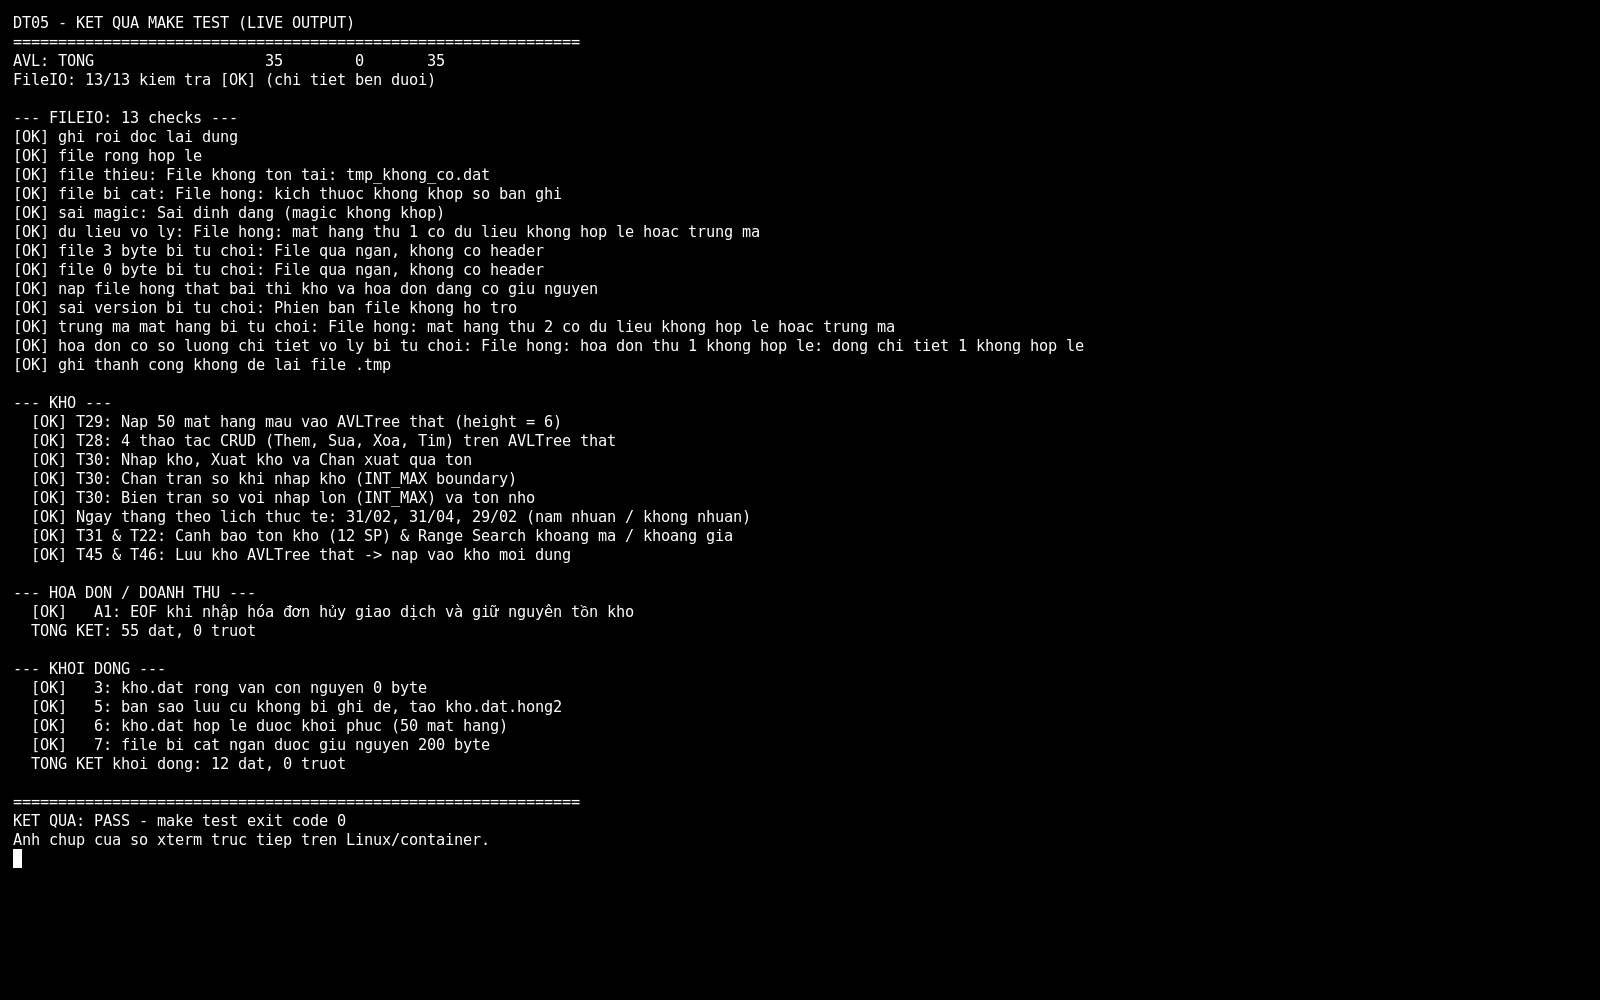
\includegraphics[width=0.98\textwidth]{console_tests.png}
\caption{Ảnh chụp xterm chạy make test trên Linux/container (không phải máy demo Windows)}
\label{fig:console_kho_test}
\end{figure}

% ============================================================================
% chuong3_doanhthu.tex - Module Hóa đơn và Doanh thu (TV4 - Hoàng Xuân Nhuật)
% ============================================================================
\section{Xây dựng Module Quản lý Hóa đơn và Doanh thu}

\subsection{Tổng quan và Phân tích Nghiệp vụ}
Trong hệ thống quản lý siêu thị, module Hóa đơn và Doanh thu đóng vai trò ghi nhận các giao dịch bán hàng thực tế, quản lý danh sách chi tiết các mặt hàng trong từng hóa đơn, đồng thời kết nối trực tiếp với Cây cân bằng AVL (\texttt{AVLTree}) nhằm tối ưu hóa hiệu năng tra cứu sản phẩm và cập nhật tồn kho. Các chức năng chính bao gồm:
\begin{enumerate}
    \item \textbf{Lập hóa đơn và Trừ tồn kho tự động:} Tra cứu mã hàng trên Cây AVL với độ phức tạp $O(\log n)$, kiểm tra điều kiện tồn kho, tính toán tổng tiền và tự động cập nhật giảm số lượng tồn trên cây theo thời gian thực.
    \item \textbf{Thống kê Doanh thu:} Tổng hợp doanh thu theo các tiêu chí thời gian (ngày, tháng) phục vụ công tác báo cáo tài chính.
    \item \textbf{Thống kê Top Mặt hàng Bán chạy:} Xây dựng thuật toán gom nhóm bằng \texttt{std::map} và sắp xếp giảm dần bằng \texttt{std::sort} để xếp hạng các mặt hàng có doanh số và số lượng tiêu thụ cao nhất.
\end{enumerate}

\subsection{Cấu trúc Dữ liệu Cốt lõi (\texttt{hoadon.h})}
Cấu trúc dữ liệu được thiết kế đồng bộ, sử dụng mảng tĩnh giới hạn tối đa 20 dòng chi tiết trong mỗi hóa đơn và kiểu dữ liệu \texttt{long long} cho các giá trị tài chính nhằm ngăn chặn hiện tượng tràn số, đồng thời tích hợp constructor khởi tạo an toàn bằng \texttt{std::memset}:

\begin{lstlisting}[language=C++, caption={Cấu trúc Dữ liệu Hóa đơn và Chi tiết (hoadon.h)}]
#ifndef HOADON_H
#define HOADON_H

#include <cstring>
#include "ngay.h"

const int MAX_CHI_TIET = 20;

struct ChiTietHoaDon {
    char maHang[16];
    int soLuongMua;
    long long donGia;

    ChiTietHoaDon() : soLuongMua(0), donGia(0) {
        std::memset(maHang, 0, sizeof(maHang));
    }
};

struct HoaDon {
    char maHoaDon[16];
    Ngay ngayLap;
    ChiTietHoaDon danhSachChiTiet[MAX_CHI_TIET];
    int soLuongChiTiet;
    long long tongTien;

    HoaDon() : ngayLap(), soLuongChiTiet(0), tongTien(0) {
        std::memset(maHoaDon, 0, sizeof(maHoaDon));
    }
};

#endif
\end{lstlisting}

\subsection{Thiết kế Nguyên mẫu Hàm (Header Modules)}

\subsubsection{Phân hệ Lập Hóa đơn và Tương tác Cây AVL (\texttt{lap\_hoa\_don.h})}
\begin{lstlisting}[language=C++, caption={Khai báo nguyên mẫu lập hóa đơn tích hợp Cây AVL}]
#ifndef LAP_HOA_DON_H
#define LAP_HOA_DON_H

#include <vector>
#include <string>
#include "mathang.h"
#include "hoadon.h"
#include "AVLTree.h"

void lapHoaDon(AVLTree<std::string, MatHang>& kho, std::vector<HoaDon>& danhSachHoaDon);
bool kiemTraHetHang(const MatHang& mh, int soLuongMua);
void truTonTuDong(MatHang& mh, int soLuongMua);
void hienThiDanhSachHoaDon(const std::vector<HoaDon>& danhSachHoaDon);

#endif
\end{lstlisting}

\subsubsection{Phân hệ Thống kê Doanh thu (\texttt{thongkedoanhthu.h})}
\begin{lstlisting}[language=C++, caption={Khai báo nguyên mẫu hàm thống kê doanh thu}]
#ifndef THONGKEDOANHTHU_H
#define THONGKEDOANHTHU_H

#include <vector>
#include "hoadon.h"
#include "ngay.h"

void thongKeDoanhThuTheoNgay(const std::vector<HoaDon>& danhSachHoaDon);
void thongKeDoanhThuTheoThang(const std::vector<HoaDon>& danhSachHoaDon);
void menuThongKeDoanhThu(const std::vector<HoaDon>& danhSachHoaDon);

#endif
\end{lstlisting}

\subsubsection{Phân hệ Thống kê Top Mặt hàng Bán chạy (\texttt{thongketop.h})}
\begin{lstlisting}[language=C++, caption={Mã nguồn chi tiết phân hệ thống kê top mặt hàng bán chạy}]
struct ThongKeMatHang {
    string maHang;
    int tongSoLuongBan;
    long long tongDoanhThuMatHang;
};

static bool soSanhBanChay(const ThongKeMatHang& a, const ThongKeMatHang& b) {
    if (a.tongSoLuongBan != b.tongSoLuongBan) {
        return a.tongSoLuongBan > b.tongSoLuongBan;
    }
    return a.tongDoanhThuMatHang > b.tongDoanhThuMatHang;
}

inline void thongKeTopMatHangBanChay(const vector<HoaDon>& danhSachHoaDon, const KhoHang& kho) {
    if (danhSachHoaDon.empty()) {
        cout << "\n[Thong bao] He thong chua co du lieu hoa don nao de thong ke!\n";
        return;
    }

    map<string, ThongKeMatHang> mapThongKe;
    for (size_t i = 0; i < danhSachHoaDon.size(); ++i) {
        const HoaDon& hd = danhSachHoaDon[i];
        for (int j = 0; j < hd.soLuongChiTiet; ++j) {
            const ChiTietHoaDon& ct = hd.danhSachChiTiet[j];
            string ma(ct.maHang);
            mapThongKe[ma].maHang = ma;
            mapThongKe[ma].tongSoLuongBan += ct.soLuongMua;
            mapThongKe[ma].tongDoanhThuMatHang += (long long)ct.soLuongMua * ct.donGia;
        }
    }

    vector<ThongKeMatHang> danhSachThongKe;
    for (map<string, ThongKeMatHang>::const_iterator it = mapThongKe.begin(); it != mapThongKe.end(); ++it) {
        danhSachThongKe.push_back(it->second);
    }
    sort(danhSachThongKe.begin(), danhSachThongKe.end(), soSanhBanChay);
    // In bang Top N mat hang ban chay va tra cuu ten hang qua kho.search(tk.maHang)
}
\end{lstlisting}

\subsubsection{Chương trình Kiểm thử Hiệu năng Benchmark (\texttt{Chuongtrinhsinhvadodulieu.h})}
\begin{lstlisting}[language=C++, caption={Chương trình sinh dữ liệu và đo đạc benchmark thực tế}]
inline void chayToanBoBenchmark() {
    std::cout << "\n==================================================\n";
    std::cout << "   CHUONG TRINH BENCHMARK HIEU NANG AVL\n";
    std::cout << "==================================================\n";

    thucHienDoBenchmark(1000);
    thucHienDoBenchmark(10000);
    thucHienDoBenchmark(100000);

    std::cout << "\n==================================================\n";
    std::cout << "Kiem thu hieu nang hoan tat thanh cong!\n";
}
\end{lstlisting}

\subsection{Giải thích Giải thuật và Thiết kế Kỹ thuật}
\begin{itemize}
    \item \textbf{Tương tác Cây AVL tối ưu $O(\log n)$:} Module lập hóa đơn sử dụng tham chiếu đến \texttt{AVLTree<string, MatHang>\& kho}, cho phép gọi phương thức \texttt{search()} để tra cứu thông tin sản phẩm và cập nhật trực tiếp lượng tồn kho trên cây với độ phức tạp đạt $O(\log n)$.
    \item \textbf{Quản lý danh sách chi tiết an toàn:} Giới hạn mảng tĩnh tối đa 20 phần tử cho mỗi hóa đơn giúp kiểm soát tốt bộ nhớ, kết hợp constructor khởi tạo an toàn bằng \texttt{std::memset} và kiểu dữ liệu \texttt{long long} cho đơn giá và tổng tiền nhằm tránh triệt để hiện tượng tràn số tài chính.
    \item \textbf{Gom nhóm và Sắp xếp hiệu quả:} Thuật toán thống kê top sử dụng \texttt{std::map<string, ThongKeMatHang>} để tự động cộng dồn số lượng và doanh thu theo từng mã hàng xuyên suốt các hóa đơn, sau đó chuyển sang \texttt{std::vector} để sắp xếp nhanh chóng thông qua hàm \texttt{std::sort}.
\end{itemize}

\section{Thiết kế và Cài đặt Module Lưu trữ File Nhị phân và Giao diện Console}

\subsection{Mục tiêu và ranh giới lưu trữ}
Module FileIO cung cấp lớp biên giữa dữ liệu đang nằm trong RAM và dữ liệu bền vững trên đĩa. Module không phụ thuộc trực tiếp vào chi tiết nút của cây AVL; hàm lưu lấy danh sách đã duyệt theo thứ tự thông qua \texttt{inorder()}, còn hàm nạp nhận lại các mặt hàng rồi gọi \texttt{clear()} và \texttt{insert()} trên cấu trúc kho. Cách thiết kế này giúp tách định dạng file khỏi cấu trúc lưu trữ đang dùng trong RAM.

\subsection{Đặc tả bố cục file}
Dữ liệu kho hàng và danh sách hóa đơn được lưu theo thứ tự tuần tự:
\[
  [\texttt{FileHeader}]\;\Vert\;[\texttt{MatHang}\times soMatHang]\;\Vert\;[\texttt{HoaDon}\times soHoaDon].
\]
Header gồm 24 byte theo định nghĩa hiện tại: 4 byte mã nhận diện \texttt{SMK1}, sau đó là các trường số nguyên 32-bit gồm phiên bản, kích thước bản ghi mặt hàng, kích thước bản ghi hóa đơn, số mặt hàng và số hóa đơn. Kích thước bản ghi được ghi trong header để phát hiện file được tạo bởi bản build có cấu trúc dữ liệu không tương thích.

\begin{figure}[H]
\centering
\begin{tikzpicture}[x=1cm,y=1cm, every node/.style={font=\small}]
  \draw[fill=blue!10] (0,0) rectangle (3.1,1.0);
  \draw[fill=green!10] (3.1,0) rectangle (8.5,1.0);
  \draw[fill=orange!12] (8.5,0) rectangle (13.5,1.0);
  \node at (1.55,0.66) {FileHeader};
  \node at (1.55,0.30) {24 byte};
  \node at (5.8,0.66) {MatHang};
  \node at (5.8,0.30) {$soMatHang$ bản ghi};
  \node at (11,0.66) {HoaDon};
  \node at (11,0.30) {$soHoaDon$ bản ghi};
  \node at (1.55,-0.35) {Magic / Version / Size / Count};
\end{tikzpicture}
\caption{Bố cục tuần tự của file kho.dat}
\label{fig:file_layout}
\end{figure}

\begin{table}[H]
\centering
\caption{Các trường trong FileHeader}
\label{tab:file_header}
\small
\begin{tabular}{@{}p{3cm}p{2.5cm}p{6.5cm}@{}}
\toprule
\textbf{Trường} & \textbf{Kiểu} & \textbf{Mục đích} \\
\midrule
\texttt{magic[4]} & 4 byte & Nhận diện định dạng file là SMK1. \\
\texttt{version} & uint32\_t & Phiên bản schema, hiện tại bằng 1. \\
\texttt{kichThuocMH} & uint32\_t & Kích thước bản ghi MatHang của bản build. \\
\texttt{kichThuocHD} & uint32\_t & Kích thước bản ghi HoaDon của bản build. \\
\texttt{soMatHang} & uint32\_t & Số bản ghi mặt hàng tiếp theo header. \\
\texttt{soHoaDon} & uint32\_t & Số bản ghi hóa đơn sau vùng mặt hàng. \\
\bottomrule
\end{tabular}
\end{table}

\subsection{Ghi dữ liệu và thay thế file}
Quy trình ghi gồm các bước: tạo file tạm có hậu tố \texttt{.tmp}; ghi header; ghi lần lượt các mặt hàng; ghi các hóa đơn; gọi \texttt{fflush}; đóng file; sau đó thay thế file đích bằng file tạm. Nếu lỗi xảy ra trong lúc ghi, file tạm được xóa và hàm trả về thông báo lỗi. Trên hệ điều hành POSIX, thao tác \texttt{rename} có thể thay thế đích trên cùng hệ thống file; trên Windows, mã nguồn dùng API thay thế file tương ứng. Cơ chế này giảm nguy cơ để lại file đích chỉ được ghi một nửa, nhưng không thay thế cho sao lưu định kỳ hoặc kiểm tra lỗi thiết bị lưu trữ.

\begin{figure}[H]
\centering
\begin{tikzpicture}[>=Latex,node distance=0.7cm,every node/.style={font=\small}]
  \node[draw,rounded corners,fill=blue!8,minimum width=3.3cm] (start) {Bắt đầu lưu};
  \node[draw,rounded corners,fill=gray!10,below=of start,minimum width=3.3cm] (tmp) {Mở kho.dat.tmp};
  \node[draw,rounded corners,fill=gray!10,below=of tmp,minimum width=3.3cm] (write) {Ghi header + bản ghi};
  \node[draw,diamond,aspect=2,fill=yellow!15,below=of write,minimum width=3.4cm] (ok) {Ghi và flush thành công?};
  \node[draw,rounded corners,fill=red!10,below left=0.8cm and 0.3cm of ok,minimum width=2.7cm] (fail) {Xóa file tạm, báo lỗi};
  \node[draw,rounded corners,fill=green!10,below right=0.8cm and 0.3cm of ok,minimum width=2.7cm] (rename) {Thay thế file đích};
  \node[draw,rounded corners,fill=blue!8,below=0.7cm of rename,minimum width=2.7cm] (done) {Hoàn tất};
  \draw[->] (start) -- (tmp);
  \draw[->] (tmp) -- (write);
  \draw[->] (write) -- (ok);
  \draw[->] (ok) -- node[above left]{Không} (fail);
  \draw[->] (ok) -- node[above right]{Có} (rename);
  \draw[->] (rename) -- (done);
\end{tikzpicture}
\caption{Quy trình ghi file qua file tạm}
\label{fig:atomic_write}
\end{figure}

\subsection{Kiểm tra khi đọc file}
Đọc file không chỉ là gọi \texttt{fread} theo số lượng được khai báo. Module xác minh lần lượt: file tồn tại; file đủ dài để chứa header; magic khớp; phiên bản được hỗ trợ; kích thước bản ghi tương thích; kích thước thực tế của file bằng tổng kích thước header và các vùng bản ghi được mô tả. Sau khi đọc, các chuỗi được ép kết thúc bằng ký tự null và dữ liệu mặt hàng được kiểm tra các thuộc tính không âm. Khi nạp vào cây, mã hàng trùng bị từ chối.

\begin{figure}[H]
\centering
\begin{tikzpicture}[>=Latex,node distance=0.55cm,every node/.style={font=\small}]
  \node[draw,rounded corners,fill=blue!8,minimum width=3.4cm] (open) {Mở file và đọc header};
  \node[draw,rounded corners,fill=gray!10,below=of open,minimum width=3.4cm] (magic) {Kiểm tra magic / version / size};
  \node[draw,rounded corners,fill=gray!10,below=of magic,minimum width=3.4cm] (length) {Đối chiếu kích thước file};
  \node[draw,rounded corners,fill=gray!10,below=of length,minimum width=3.4cm] (records) {Đọc bản ghi và kiểm tra dữ liệu};
  \node[draw,rounded corners,fill=green!10,below=of records,minimum width=3.4cm] (load) {Nạp vào AVL và danh sách hóa đơn};
  \draw[->] (open) -- (magic);
  \draw[->] (magic) -- node[right]{Hợp lệ} (length);
  \draw[->] (length) -- node[right]{Khớp} (records);
  \draw[->] (records) -- node[right]{Hợp lệ} (load);
\end{tikzpicture}
\caption{Các bước kiểm tra tính hợp lệ khi nạp file}
\label{fig:read_validation}
\end{figure}

\subsection{Xử lý lỗi và bảo đảm trạng thái nhất quán}
Hàm \texttt{napDuLieu} đọc và kiểm tra dữ liệu vào các vector tạm trước khi xóa nội dung kho hiện tại. Nếu \texttt{docFile} thất bại, kho và danh sách hóa đơn đang sử dụng không bị thay đổi. Đây là nguyên tắc quan trọng: chỉ thay thế trạng thái hoạt động sau khi dữ liệu đọc đã vượt qua các bước kiểm tra định dạng. Những lỗi được kiểm tra trong bộ test hiện tại gồm file không tồn tại, file bị cắt cụt, magic sai và dữ liệu mặt hàng không hợp lệ. Khi mở rộng hệ thống, nên bổ sung kiểm tra ngày tháng, mã hóa đơn trùng, tổng tiền và tham chiếu chi tiết hóa đơn đến mã mặt hàng.

\subsection{Mẫu mã kiểm tra header và độ dài file}
\begin{lstlisting}[language=C++,caption={Minh họa các điều kiện kiểm tra cấu trúc file}]
if (std::memcmp(h.magic, MAGIC, 4) != 0) {
    loi = "Sai dinh dang (magic khong khop)";
    return false;
}
if (h.version != VERSION) {
    loi = "Phien ban file khong ho tro";
    return false;
}
uint64_t expected = sizeof(FileHeader)
    + uint64_t(h.soMatHang) * sizeof(MatHang)
    + uint64_t(h.soHoaDon) * sizeof(HoaDon);
if (expected != uint64_t(size)) {
    loi = "File hong: kich thuoc khong khop";
    return false;
}
\end{lstlisting}

\subsection{Giao diện Menu Console}
Giao diện console được chia thành menu chính và các menu con: quản lý kho; hóa đơn/doanh thu; lưu trữ; chạy benchmark; xem nhanh cảnh báo. Menu chính hiển thị số lượng mặt hàng, chiều cao cây và số hóa đơn hiện có để người dùng có phản hồi về trạng thái chương trình. Mỗi menu con nhận lựa chọn từ hàm đọc số nguyên có kiểm tra miền giá trị.

Nếu người dùng nhập ký tự thay vì số, luồng \texttt{std::cin} chuyển sang trạng thái lỗi. Chương trình gọi \texttt{cin.clear()} để khôi phục trạng thái và \texttt{cin.ignore()} để bỏ phần còn lại của dòng. Nếu không xử lý hai bước này, các lần đọc sau có thể tiếp tục thất bại trên cùng dữ liệu lỗi, tạo cảm giác chương trình bị treo.

\subsection{Xử lý ngoại lệ và vòng đời bộ nhớ}
Khối \texttt{main()} được đặt trong \texttt{try/catch} để chuyển các ngoại lệ chưa xử lý thành thông báo có kiểm soát. Cây AVL có destructor giải phóng các nút khi đối tượng rời khỏi phạm vi. Việc thu hồi bộ nhớ theo RAII giảm nguy cơ rò rỉ khi kết thúc chương trình bình thường; tuy nhiên, khẳng định không có rò rỉ trong mọi đường chạy cần được kiểm tra riêng bằng công cụ chuyên dụng như AddressSanitizer hoặc Valgrind trên môi trường phù hợp. Báo cáo không xem sự tồn tại của destructor là bằng chứng thay thế cho kiểm thử bộ nhớ.

\subsection{Kiểm thử FileIO và các giới hạn}
Bộ kiểm thử FileIO hiện thực các ca: ghi rồi đọc lại dữ liệu; xử lý file rỗng hợp lệ; từ chối file không tồn tại; từ chối file bị cắt; từ chối magic sai; từ chối bản ghi mặt hàng có giá trị vô lý. Phần kiểm thử tích hợp kho còn xác nhận có thể lưu danh sách mặt hàng và hóa đơn rồi nạp lại vào một cây AVL khác.

Định dạng hiện tại ghi trực tiếp biểu diễn nhị phân của struct, vì vậy kích thước và cách bố trí struct phụ thuộc compiler, ABI và cách căn chỉnh bộ nhớ. Header chứa kích thước struct giúp phát hiện một số trường hợp không tương thích nhưng không tạo ra định dạng di động tuyệt đối giữa mọi nền tảng. Một phiên bản nâng cấp nên ghi từng trường theo thứ tự và quy ước byte cụ thể, có checksum, giới hạn số bản ghi, và cơ chế chuyển đổi schema khi đổi phiên bản.

\begin{table}[H]
\centering
\caption{Các ca kiểm thử FileIO đã chạy}
\label{tab:test_fileio}
\small
\begin{tabular}{@{}p{1cm}p{4cm}p{6cm}p{2.5cm}@{}}
\toprule
\textbf{Mã} & \textbf{Tình huống} & \textbf{Kết quả mong đợi} & \textbf{Kết quả chạy} \\
\midrule
F01 & Ghi và đọc lại & Dữ liệu mặt hàng/hóa đơn giữ nguyên. & Đạt \\
F02 & File rỗng & Đọc thành công với hai danh sách rỗng. & Đạt \\
F03 & File không tồn tại & Trả lỗi, không làm thay đổi kho. & Đạt \\
F04 & File bị cắt & Từ chối do kích thước không khớp. & Đạt \\
F05 & Magic sai & Từ chối do định dạng không khớp. & Đạt \\
F06 & Dữ liệu âm/vô lý & Từ chối bản ghi. & Đạt \\
\bottomrule
\end{tabular}
\end{table}

\subsection{Hướng dẫn thao tác demo}
Để minh họa module, người trình bày chạy \texttt{./main\_app}, kiểm tra thông báo nạp CSV ban đầu, mở menu lưu trữ và thực hiện lưu dữ liệu. Sau đó có thể thoát và chạy lại chương trình để quan sát cơ chế phục hồi từ file. Một ca kiểm thử lỗi nên chạy độc lập trong bộ test FileIO thay vì cố làm hỏng file dữ liệu đang dùng cho demo. Khi trình bày, cần phân biệt rõ dữ liệu mẫu CSV dùng khởi tạo lần đầu với file nhị phân dùng lưu trạng thái sau giao dịch. Khi khởi động, \texttt{main} phân biệt ba tình huống: (1) \texttt{kho.dat} đọc được thì khôi phục dữ liệu; (2) \texttt{kho.dat} chưa tồn tại thì nạp dữ liệu mẫu CSV; (3) \texttt{kho.dat} tồn tại nhưng không đọc được thì báo lỗi kèm lý do và \textbf{không tự ghi đè}. Ở tình huống (3), người dùng chọn thoát để giữ nguyên file, hoặc chọn sao lưu file lỗi thành \texttt{kho.dat.hongN} (không bao giờ ghi đè bản sao lưu cũ) rồi mới dùng dữ liệu mẫu; nếu sao lưu thất bại thì chương trình dừng. Hàm kiểm tra sự tồn tại chỉ coi là "chưa có file" khi hệ điều hành báo \texttt{ENOENT}; mọi lỗi khác (không có quyền đọc, đường dẫn là thư mục) đều đi vào nhánh báo lỗi. Kịch bản này được kiểm thử tự động bằng \texttt{tests/test\_khoi\_dong.sh} trong thư mục tạm, không đụng tới \texttt{kho.dat} thật.


\subsection{Đầu ra kiểm thử và cách đọc thông báo}
Trong bản ghi kiểm thử, thông báo bắt đầu bằng \texttt{[OK]} biểu thị ca kiểm thử đã đạt. Một số dòng có tiền tố \texttt{[Lỗi]} được tạo có chủ đích để xác nhận chương trình từ chối dữ liệu không hợp lệ; đó không phải lỗi làm hỏng tiến trình test. Khi báo cáo kết quả, cần phân biệt lỗi nghiệp vụ được kiểm tra với lỗi assertion thực sự.


% ============================================================================
% Chuong 4 - ket qua benchmark chay lai tren cung mot moi truong
% ============================================================================
\chapter{Thực nghiệm và Đánh giá Hiệu năng}

\section{Mục tiêu thực nghiệm}
Chương này so sánh chi phí tìm kiếm chính xác theo mã hàng của cây AVL với vector đã sắp xếp sử dụng \texttt{std::lower\_bound}. Đây là baseline công bằng hơn so với duyệt tuyến tính: cả hai phương pháp đều khai thác thứ tự khóa và có số phép so sánh tăng theo logarithm. Ngoài tìm kiếm, benchmark đo riêng 100 lần chèn và 100 lần xóa để thể hiện chi phí cập nhật của hai cấu trúc.

\section{Môi trường và phương pháp đo}
Lần chạy được thực hiện ngày 31/10/2026 trong môi trường Linux x86\_64, nhân 6.18.57, GCC 14.2.0, 3 CPU logic được cấp cho container; cờ biên dịch là \texttt{-std=c++11 -O2 -Wall -Wextra}. Đây là môi trường ảo hóa/container, không phải phép đo trên máy demo của nhóm. Vì vậy, thời gian tuyệt đối có thể khác trên máy cá nhân hoặc máy giảng viên.

Chương trình tạo lần lượt 1.000, 10.000, 50.000 và 100.000 mặt hàng. Cả AVL và vector được nạp cùng tập mã khóa. Vector luôn được duy trì theo thứ tự tăng dần; tìm kiếm dùng \texttt{lower\_bound}. Một tập 1.000 khóa đã tồn tại, được sinh bằng \texttt{std::mt19937} với seed 2026, được dùng chung cho hai cấu trúc. Sau một lượt làm nóng, mỗi phương pháp được đo 9 lần bằng \texttt{steady\_clock}; báo cáo lấy trung vị thời gian tổng của 1.000 truy vấn. Chèn và xóa cũng được đo riêng: mỗi lượt gồm 100 thao tác trên bản sao dữ liệu đã chuẩn bị trước, đo 9 lần và lấy trung vị. Thời gian khởi tạo/copy cấu trúc không được tính vào khoảng đo cập nhật.

\section{Kết quả đo tìm kiếm}
Bảng~\ref{tab:benchmark_search} trình bày trung vị tổng thời gian của 1.000 truy vấn. Tất cả truy vấn đều tìm thấy khóa tương ứng ở cả hai cấu trúc.

\begin{table}[H]
\centering
\caption{Trung vị thời gian tìm kiếm 1.000 khóa (9 lần đo)}
\label{tab:benchmark_search}
\small
\begin{tabular}{@{}rrrrr@{}}
\toprule
\textbf{Số mặt hàng} & \textbf{Chiều cao AVL} & \textbf{AVL ($\mu$s)} & \textbf{Vector + lower\_bound ($\mu$s)} & \textbf{Vector/AVL} \\
\midrule
1.000   & 10 & 100,089 & 64,496  & 0,64 lần \\
10.000  & 14 & 192,745 & 122,081 & 0,63 lần \\
50.000  & 16 & 284,702 & 187,238 & 0,66 lần \\
100.000 & 17 & 389,176 & 216,581 & 0,56 lần \\
\bottomrule
\end{tabular}
\end{table}

\section{Kết quả đo chèn và xóa}
Bảng~\ref{tab:benchmark_update} ghi nhận tổng thời gian của 100 thao tác chèn hoặc xóa. Các thao tác trên vector dùng tìm vị trí bằng \texttt{lower\_bound}, sau đó \texttt{insert}/\texttt{erase} phải dịch chuyển phần tử để giữ thứ tự.

\begin{table}[H]
\centering
\caption{Trung vị thời gian của 100 thao tác cập nhật (9 lần đo)}
\label{tab:benchmark_update}
\small
\begin{tabular}{@{}rrrrrr@{}}
\toprule
\textbf{Số mặt hàng} & \textbf{AVL chèn ($\mu$s)} & \textbf{Vector chèn ($\mu$s)} & \textbf{AVL xóa ($\mu$s)} & \textbf{Vector xóa ($\mu$s)} \\
\midrule
1.000   & 10,816 & 323,700   & 12,438  & 188,830 \\
10.000  & 14,231 & 4.321,075 & 32,068  & 2.181,564 \\
50.000  & 21,362 & 21.464,294 & 129,231 & 10.705,357 \\
100.000 & 23,595 & 40.817,120 & 177,273 & 21.948,953 \\
\bottomrule
\end{tabular}
\end{table}

\section{Trực quan hóa kết quả tìm kiếm}
Biểu đồ~\ref{fig:chart_tv4} so sánh hai phương pháp tìm kiếm bằng thang logarit. Vector đã sắp xếp nhanh hơn trong lần chạy này, dù cả hai phương pháp đều có độ phức tạp tìm kiếm logarithm theo số phần tử.

\begin{figure}[H]
\centering
\begin{tikzpicture}
\begin{axis}[
  ybar, bar width=13pt, width=0.92\textwidth, height=8cm,
  ylabel={Thời gian cho 1.000 truy vấn ($\mu$s, log)},
  xlabel={Quy mô dữ liệu}, symbolic x coords={1k,10k,50k,100k}, xtick=data,
  ymode=log, log basis y=10, ymin=30, ymax=400,
  legend style={at={(0.5,-0.2)},anchor=north,legend columns=2},
  grid=major, enlarge x limits=0.2
]
\addplot coordinates {(1k,100.089) (10k,192.745) (50k,284.702) (100k,389.176)};
\addplot coordinates {(1k,64.496) (10k,122.081) (50k,187.238) (100k,216.581)};
\legend{AVL, Vector + lower\_bound}
\end{axis}
\end{tikzpicture}
\caption{So sánh thời gian tìm kiếm bằng AVL và vector đã sắp xếp}
\label{fig:chart_tv4}
\end{figure}

\section{Phân tích kết quả và liên hệ độ phức tạp}
Ở quy mô 100.000 mặt hàng, AVL có chiều cao 17 và cần 389,176 $\mu$s cho 1.000 truy vấn; vector đã sắp xếp với \texttt{lower\_bound} cần 216,581 $\mu$s. Trong lần đo này, vector nhanh hơn khoảng 1,79 lần. Kết quả không mâu thuẫn với độ phức tạp lý thuyết: tìm kiếm trên AVL là $O(\log n)$ theo chiều cao cây, còn tìm kiếm nhị phân trên vector đã sắp xếp cũng là $O(\log n)$.

Chênh lệch thời gian thực tế chịu ảnh hưởng của hằng số chi phí và kiến trúc bộ nhớ. Vector lưu phần tử liên tục nên tận dụng locality/cache tốt hơn; thao tác nhị phân thường truy cập ít vùng nhớ và không cần lần theo con trỏ node. AVL phải đi qua các node được cấp phát rời rạc, nên pointer chasing và cache miss có thể làm tăng độ trễ dù chiều cao cây nhỏ. Do vậy, không thể kết luận rằng AVL luôn nhanh hơn vector trong mọi tác vụ chỉ dựa vào ký hiệu $O(\log n)$.

Ở chiều ngược lại, cập nhật trên vector phải dịch chuyển các phần tử để duy trì thứ tự. Tại 100.000 mặt hàng, 100 lần chèn mất 40.817,120 $\mu$s trên vector so với 23,595 $\mu$s trên AVL; 100 lần xóa mất 21.948,953 $\mu$s trên vector so với 177,273 $\mu$s trên AVL. Số đo cho thấy cấu trúc phù hợp phụ thuộc vào tỷ lệ đọc/ghi: vector có lợi thế tra cứu trong bộ nhớ liên tục, còn cây AVL phù hợp hơn khi cần cập nhật thường xuyên và duy trì thứ tự khóa.

\section{Giới hạn của phép đo}
Kết quả là trung vị của 9 lần đo trong một môi trường container, với một bộ dữ liệu và các truy vấn thành công. Benchmark chưa đo truy vấn không tìm thấy, RAM, cấp phát bộ nhớ, lưu file, tải đồng thời, hoặc độ trễ từ thao tác người dùng. Mức nhiễu do lịch CPU, cache, compiler và cấu hình máy vẫn có thể ảnh hưởng. Vì vậy, số liệu chỉ mô tả lần chạy kèm gói bàn giao, không phải cam kết hiệu năng trên máy khác.

\section{Trích xuất đầu ra benchmark}
Đầu ra stdout thực tế của lần chạy được lưu tại \texttt{benchmark\_console.txt}. Có thể đối chiếu trực tiếp các giá trị trong bảng với tệp log này.
\lstinputlisting[caption={Trích đoạn stdout của lần benchmark đã chạy},firstline=1,lastline=42]{benchmark_console.txt}

\section{Kết luận chương}
Trong lần thực nghiệm này, AVL và vector đã sắp xếp có hiệu năng tìm kiếm cùng mức độ tăng trưởng logarithm; vector nhanh hơn về tra cứu nhờ tính cục bộ bộ nhớ, trong khi AVL có lợi thế rõ rệt ở các phép cập nhật được đo. AVL vẫn là cấu trúc lõi phù hợp với yêu cầu quản lý kho có thêm/xóa mặt hàng, nhưng quyết định cuối cùng cần xét đồng thời tỷ lệ đọc/ghi, bộ nhớ và yêu cầu nghiệp vụ.


\chapter*{Kết luận}
\addcontentsline{toc}{chapter}{Kết luận}

\section*{Kết quả đạt được}
Nhóm đã xây dựng bản tích hợp hệ thống quản lý hàng tồn kho và doanh thu siêu thị sử dụng cây AVL tự cài đặt làm cấu trúc dữ liệu lõi. Trên phiên bản mã nguồn được ghép từ năm gói thành viên và cập nhật trong đợt này, các kết quả có thể kiểm chứng gồm:
\begin{itemize}
  \item Cài đặt \texttt{AVLTree<K,V>} với thêm, xóa, tìm kiếm, duyệt, range search, kích thước/chiều cao và kiểm tra rỗng. Bộ kiểm thử cập nhật đạt 35/35 ca, trong đó có kiểm tra tính \texttt{const} của kết quả tìm kiếm và move constructor/assignment.
  \item Module kho hỗ trợ CRUD, nhập/xuất, chặn xuất quá tồn, kiểm tra tràn số khi nhập, kiểm tra ngày theo lịch và nạp CSV có xác thực từng dòng. Các kịch bản tích hợp kho hiện có chạy đạt.
  \item Module hóa đơn chỉ trừ tồn sau khi người dùng xác nhận toàn bộ giao dịch; EOF hoặc từ chối xác nhận hủy hóa đơn và giữ nguyên tồn kho. Mã hóa đơn trùng, số lượng không hợp lệ, dòng hàng lặp và tổng tiền vượt giới hạn được kiểm tra. Bộ test hóa đơn--doanh thu đạt 55/55 ca.
  \item Module FileIO kiểm tra magic/version, kích thước, mã hàng trùng, trường dữ liệu mặt hàng và chi tiết hóa đơn; khi ghi, vùng đệm của struct được khởi tạo trước khi tuần tự hóa. Các ca FileIO được mở rộng và chạy đạt.
  \item Makefile đã theo dõi phụ thuộc header qua \texttt{-MMD -MP}, có target \texttt{asan}; bộ test khởi động đạt 12/12 ca và xác nhận file kho hỏng không bị tự động ghi đè.
\end{itemize}

\section*{Kết quả benchmark}
Lần benchmark cập nhật ngày 31/10/2026 chạy với GCC 14.2.0 trên Linux x86\_64, container được cấp 3 CPU logic. Mỗi cấu trúc thực hiện cùng 1.000 truy vấn; chạy làm nóng trước, đo 9 lần và lấy trung vị. Ở 100.000 mặt hàng, AVL có chiều cao 17 và mất 389,176 $\mu$s; vector đã sắp xếp với \texttt{lower\_bound} mất 216,581 $\mu$s cho 1.000 truy vấn. Như vậy vector nhanh hơn khoảng 1,79 lần trong phép đo tìm kiếm này, phù hợp với lợi thế locality/cache của vùng nhớ liên tục; cả hai phương pháp đều có chi phí tìm kiếm logarithm.

Với 100 thao tác cập nhật tại 100.000 mặt hàng, AVL mất 23,595 $\mu$s cho chèn và 177,273 $\mu$s cho xóa; vector đã sắp xếp lần lượt mất 40.817,120 $\mu$s và 21.948,953 $\mu$s do phải dịch chuyển phần tử. Kết quả cho thấy không thể kết luận AVL luôn nhanh hơn trong mọi tác vụ; lợi thế của mỗi cấu trúc phụ thuộc vào tỷ lệ tra cứu/cập nhật. Các bảng và phương pháp đo chi tiết nằm ở Chương 4, dữ liệu stdout được lưu trong \texttt{benchmark\_console.txt}.

\section*{Hạn chế}
\begin{itemize}
  \item Ứng dụng vẫn là giao diện console, chưa có xác thực, phân quyền hoặc giao diện đồ họa.
  \item Dữ liệu kho được lưu bằng định dạng nhị phân gắn với cách bố trí struct của bản build; chưa phải định dạng trao đổi độc lập nền tảng.
  \item Tra cứu theo khoảng giá vẫn phải duyệt dữ liệu vì cây AVL hiện được khóa theo mã hàng; chưa có chỉ mục phụ theo giá.
  \item Mỗi hóa đơn giới hạn tối đa 20 dòng chi tiết.
  \item Benchmark được thực hiện trong một môi trường container và với một bộ truy vấn; chưa đánh giá RAM, truy vấn thất bại, tải đồng thời hay thời gian lưu file.
\end{itemize}

\section*{Công việc cần xác nhận trước khi nộp}
Các gói file có thể chứng minh mã nguồn, nội dung LaTeX, slide, kịch bản demo và kết quả build/test trong môi trường hiện tại. Tuy nhiên, chúng không cung cấp lịch sử commit, dữ liệu Jira, URL/trạng thái pull request, email gửi giảng viên, biên nhận nộp bài hoặc biên bản tập dượt/đọc chéo. Vì vậy, nhóm cần thực hiện và lưu những bằng chứng này trực tiếp trước khi đánh dấu các task quy trình là hoàn tất. Tỷ lệ đóng góp của từng người phải được tính từ commit và công việc thực tế, không tự đặt mặc định.

\section*{Hướng phát triển}
Các hướng mở rộng gồm xây dựng chỉ mục phụ theo đơn giá; chuyển sang cơ sở dữ liệu có giao dịch; chuẩn hóa định dạng lưu file độc lập ABI và có checksum; thêm kiểm thử bộ nhớ; bổ sung tìm kiếm theo tên/nhóm hàng; xây dựng giao diện đồ họa hoặc web; và mở rộng benchmark sang truy vấn thất bại, bộ nhớ, tải đồng thời cũng như các phân phối dữ liệu khác.


\begin{thebibliography}{9}
\bibitem{clrs} T. H. Cormen, C. E. Leiserson, R. L. Rivest, C. Stein, \textit{Introduction to Algorithms}, 4th ed., MIT Press, 2022.
\bibitem{adelson} G. M. Adelson-Velsky, E. M. Landis, ``An algorithm for the organization of information'', \textit{Doklady Akademii Nauk SSSR}, 146, 1962.
\bibitem{knuth} D. E. Knuth, \textit{The Art of Computer Programming, Vol. 3: Sorting and Searching}, 2nd ed., Addison-Wesley, 1998.
\bibitem{stroustrup} B. Stroustrup, \textit{The C++ Programming Language}, 4th ed., Addison-Wesley, 2013.
\end{thebibliography}

\chapter*{Phụ lục: Phân công công việc và tình trạng xác minh}
\addcontentsline{toc}{chapter}{Phụ lục: Phân công công việc và tình trạng xác minh}

Bảng dưới đây mô tả phạm vi công việc được phân công trong kế hoạch và các tệp bàn giao có trong gói hiện tại. Tỷ lệ đóng góp thực tế không được suy ra từ số lượng file hoặc số task được giao. Cần đối chiếu lịch sử commit, nội dung pull request và trạng thái Jira trước khi ghi nhận phần trăm đóng góp chính thức.

\begin{table}[H]
\centering
\caption{Phạm vi phân công và bằng chứng trong gói bàn giao}
\begin{tabular}{@{}p{2.5cm}p{2.5cm}p{5.2cm}p{1.5cm}p{1.8cm}@{}}
\toprule
\textbf{Thành viên} & \textbf{Nhánh dự kiến} & \textbf{Phạm vi chính} & \textbf{Task} & \textbf{Tỷ lệ thực tế} \\
\midrule
TV1 -- Đoàn Quốc Nhật & \texttt{main-integration} & Tích hợp, Makefile, chương trình chính, khung và kết luận báo cáo. & T01--T15 & Chưa xác minh \\
TV2 -- Huỳnh Long Nhật & \texttt{avl-tree} & Cây AVL, bộ test cấu trúc dữ liệu, Chương 2. & T16--T25 & Chưa xác minh \\
TV3 -- Trần Văn Tài & \texttt{module-kho} & Module kho, dữ liệu mẫu, Chương 1 và phần kho Chương 3. & T26--T34 & Chưa xác minh \\
TV4 -- Hoàng Xuân Nhuật & \texttt{module-doanh-thu} & Hóa đơn, doanh thu, benchmark, Chương 4. & T35--T43 & Chưa xác minh \\
TV5 -- Nguyễn Duy Khang & \texttt{fileio-ui} & FileIO, giao diện console, slide và kịch bản demo. & T44--T52 & Chưa xác minh \\
Cả nhóm & \texttt{main} & Đọc chéo báo cáo và tập dượt demo. & T52--T53 & Cần biên bản \\
\bottomrule
\end{tabular}
\end{table}

\section*{Quy tắc xác nhận phần trăm đóng góp}
Khi hoàn thiện phụ lục cuối cùng, nhóm nên thống nhất một khoảng thời gian thống kê; xuất danh sách commit theo từng tác giả; loại commit merge, commit bot và commit trùng lặp; đối chiếu thay đổi thực chất của từng pull request; sau đó so sánh với task Jira đã được nghiệm thu. Số dòng thêm/xóa không nên là tiêu chí duy nhất vì một thay đổi thiết kế hoặc sửa lỗi nhỏ có thể có giá trị khác với việc sinh mã tự động.

\section*{Danh sách minh chứng quy trình cần lưu}
\begin{itemize}
  \item Đường dẫn repository và ảnh/chụp xuất lịch sử commit theo thành viên.
  \item Link pull request, người review, ngày merge và trạng thái cuối của từng nhánh.
  \item Bản xuất Jira thể hiện assignee, deadline, trạng thái và người nghiệm thu cho các task.
  \item Email hoặc xác nhận chia sẻ bản LaTeX cho giảng viên (T04).
  \item Phiếu/biên bản đọc chéo báo cáo của các thành viên (T53).
  \item Biên bản tập dượt demo hoặc checklist chạy thử có người tham gia (T52).
\end{itemize}

Không có các minh chứng trên trong các tệp được cung cấp ở lần rà soát này. Vì vậy, phụ lục sử dụng nhãn ``chưa xác minh'' thay vì ghi 20\% đồng đều cho từng thành viên.

\chapter*{Phụ lục: Hướng dẫn biên dịch, kiểm thử và nghiệm thu}
\addcontentsline{toc}{chapter}{Phụ lục: Hướng dẫn biên dịch, kiểm thử và nghiệm thu}

\section*{A. Cấu trúc thư mục bàn giao}
Dự án được chia thành các thư mục theo trách nhiệm kỹ thuật. Thư mục \texttt{include/} chứa khai báo cấu trúc và giao diện module; \texttt{src/} chứa các định nghĩa hàm và điểm vào chương trình; \texttt{tests/} chứa bộ kiểm thử; \texttt{data/} chứa dữ liệu CSV mẫu; \texttt{docs/baocao/} chứa các tệp LaTeX; \texttt{docs/demo\_slide/} chứa slide và kịch bản demo. Cấu trúc này giúp phân biệt mã chạy, mã kiểm thử và tài liệu.

\begin{table}[H]
\centering
\caption{Các tệp nguồn chính trong dự án tích hợp}
\small
\begin{tabular}{@{}p{4cm}p{3cm}p{6cm}@{}}
\toprule
\textbf{Tệp} & \textbf{Vai trò} & \textbf{Ghi chú} \\
\midrule
\texttt{include/AVLTree.h}, \texttt{AVLTree.tpp} & Cấu trúc AVL & Giao diện và phần cài đặt template. \\
\texttt{include/mathang.h} & Mô hình mặt hàng & Kiểu dữ liệu dùng chung. \\
\texttt{src/quan\_ly\_kho.cpp} & Nghiệp vụ kho & CRUD, nhập/xuất, cảnh báo, nạp CSV. \\
\texttt{src/lap\_hoa\_don.cpp} & Hóa đơn & Kiểm tra tồn và trừ tồn. \\
\texttt{src/thongkedoanhthu.cpp} & Thống kê & Doanh thu ngày/tháng. \\
\texttt{include/FileIO.h} & Lưu trữ & Ghi và đọc file nhị phân. \\
\texttt{src/main.cpp} & Giao diện & Điều phối menu và module. \\
\texttt{src/benchmark.cpp} & Benchmark & Chạy phép so sánh AVL/vector độc lập. \\
\bottomrule
\end{tabular}
\end{table}

\section*{B. Các lệnh biên dịch và kiểm thử}
Các lệnh dưới đây được chạy từ thư mục gốc repository. Cần có trình biên dịch GCC hỗ trợ C++11 và công cụ \texttt{make}. Build có thể thực hiện như sau:
\begin{lstlisting}[language=bash,caption={Biên dịch toàn bộ chương trình}]
make clean
make
\end{lstlisting}
Lệnh \texttt{make} tạo \texttt{main\_app} và \texttt{benchmark\_app}. Chương trình chính có thể chạy bằng:
\begin{lstlisting}[language=bash,caption={Chạy menu và chương trình benchmark}]
./main_app
./benchmark_app
\end{lstlisting}
Bộ test tích hợp được biên dịch và chạy bằng:
\begin{lstlisting}[language=bash,caption={Chạy các nhóm kiểm thử và tích hợp}]
make test
\end{lstlisting}
Khi kiểm tra thủ công, nên bắt đầu ở thư mục gốc để đường dẫn tương đối tới \texttt{data/du\_lieu\_mau.csv} được phân giải đúng. Không nên chạy trực tiếp từ thư mục \texttt{src/} vì các đường dẫn tương đối của ứng dụng được thiết kế theo gốc repository.

\section*{C. Ma trận độ phức tạp thao tác}
Bảng dưới đây tóm tắt độ phức tạp theo cấu trúc hiện tại. Ký hiệu $n$ là số mặt hàng, $k$ là số kết quả trong khoảng khóa, $d$ là số hóa đơn và $c$ là tổng số dòng chi tiết của các hóa đơn được duyệt.
\begin{table}[H]
\centering
\caption{Độ phức tạp của các thao tác chính}
\small
\begin{tabular}{@{}p{4.2cm}p{2.1cm}p{6.5cm}@{}}
\toprule
\textbf{Thao tác} & \textbf{Độ phức tạp} & \textbf{Giải thích} \\
\midrule
Tìm kiếm theo mã & $O(\log n)$ & Đi theo một nhánh cây AVL. \\
Thêm mặt hàng & $O(\log n)$ & Tìm vị trí chèn và cập nhật cân bằng. \\
Xóa mặt hàng & $O(\log n)$ & Tìm nút, xóa và cân bằng đường đi lên gốc. \\
Duyệt toàn bộ kho & $O(n)$ & Mỗi nút được thăm đúng một lần. \\
Range search theo mã & $O(\log n+k)$ & Tìm vùng bắt đầu và duyệt các nút thuộc đoạn. \\
Lọc theo khoảng giá & $O(n)$ & Duyệt toàn bộ vì cây không khóa theo giá. \\
Lập hóa đơn có $r$ dòng & $O(r\log n)$ & Mỗi dòng tìm một mã hàng trong cây; bỏ qua chi phí nhập/xuất console. \\
Cảnh báo tồn tối thiểu & $O(n)$ & Kiểm tra điều kiện trên toàn bộ mặt hàng. \\
Lưu kho và hóa đơn & $O(n+d+c)$ & Ghi toàn bộ bản ghi mặt hàng, hóa đơn và chi tiết. \\
Nạp file và dựng cây & $O(n\log n+d+c)$ & Đọc bản ghi rồi chèn từng mặt hàng vào AVL. \\
\bottomrule
\end{tabular}
\end{table}

Các độ phức tạp nêu trên là mô tả số thao tác theo kích thước đầu vào, không bao gồm chi phí nhập xuất console hoặc thời gian truy cập thiết bị lưu trữ cụ thể. Khi cần phân tích thực tế, phải đo riêng từng tác vụ và mô tả kích thước đầu vào tương ứng.

\section*{D. Bảng kiểm thử nghiệm thu}
\begin{table}[H]
\centering
\caption{Checklist các bằng chứng kỹ thuật được ghi nhận}
\small
\begin{tabular}{@{}p{3cm}p{6.7cm}p{3cm}@{}}
\toprule
\textbf{Nhóm} & \textbf{Bằng chứng trong lần kiểm tra} & \textbf{Kết quả} \\
\midrule
Build & \texttt{make clean} và \texttt{make} với GCC 14.2.0, C++11, \texttt{-O2}. & Thành công \\
AVL & 12 phép quay, 12 ca xóa, 2 ca const/move, 9 ca range search. & 35/35 đạt \\
FileIO & Ghi/đọc, file rỗng, file thiếu, file cụt, magic/version sai, dữ liệu mặt hàng vô lý, mã trùng, chi tiết hóa đơn không hợp lệ; file 3 byte và 0 byte bị từ chối; nạp file hỏng không làm đổi kho đang có. & 13 kiểm tra đạt \\
Kho & Nạp CSV, CRUD, nhập/xuất, chặn vượt tồn, chặn tràn \texttt{INT\_MAX} khi nhập kho, ngày theo lịch thực tế (31/02, 31/04, năm nhuận), cảnh báo, range search, lưu/nạp. & Các assertion đạt \\
Hóa đơn & Lập hóa đơn theo giao dịch; EOF/hủy xác nhận không trừ kho; mã trùng, lặp mã hàng, tổng tiền tràn; thống kê ngày/tháng. & 55/55 đạt \\
Khởi động & \texttt{tests/test\_khoi\_dong.sh}: chưa có \texttt{kho.dat}; file 3 byte / 0 byte / bị cắt không bị ghi đè; sao lưu \texttt{kho.dat.hongN}; khôi phục file hợp lệ. & 12/12 đạt \\
Benchmark & 4 quy mô; 1.000 truy vấn; 9 lần đo; vector sorted + lower\_bound và 100 chèn/xóa. & Có bảng, biểu đồ và stdout \\
Báo cáo & Hai lượt XeLaTeX, rà soát PDF và số trang sau khi ghép phụ lục. & 42 trang A4 \\
Sanitizer & \texttt{make asan} với AddressSanitizer và UndefinedBehaviorSanitizer; tất cả test chạy qua. & Thành công \\
\bottomrule
\end{tabular}
\end{table}

Các trạng thái trên chỉ phản ánh các lệnh đã chạy trong môi trường kiểm tra của lần bàn giao này. Chúng không chứng minh rằng pull request đã được merge trên GitHub, task đã được cập nhật trên Jira hoặc giảng viên đã nhận được bản LaTeX.

\section*{E. Checklist thao tác demo}
Trình tự demo nên được tiến hành trên một bản build sạch để tránh sử dụng file nhị phân từ lần chạy cũ:
\begin{enumerate}
  \item Chạy \texttt{make clean} rồi \texttt{make}; xác nhận hai executable được tạo.
  \item Chạy \texttt{./main\_app}; quan sát thông báo nạp 50 mặt hàng CSV nếu chưa tồn tại \texttt{kho.dat}.
  \item Mở phân hệ kho; duyệt danh sách theo mã; tìm một mã có thật và một mã không có.
  \item Thêm mã mới; thử thêm lại cùng mã để trình bày cơ chế từ chối trùng.
  \item Thử xuất vượt tồn và xác nhận số lượng tồn không bị thay đổi; tiếp đó xuất một lượng hợp lệ.
  \item Mở phân hệ hóa đơn; lập hóa đơn nhỏ với một hoặc hai mặt hàng; đối chiếu tổng tiền và tồn sau bán.
  \item Lưu dữ liệu; thoát chương trình; mở lại để xác nhận phục hồi từ file nhị phân.
  \item Trình bày cơ chế bảo vệ dữ liệu: chạy \texttt{sh tests/test\_khoi\_dong.sh} để kiểm tra \texttt{kho.dat} hỏng không bị ghi đè (script chạy trong thư mục tạm, không làm hỏng file dữ liệu của buổi demo).
  \item Chạy \texttt{./benchmark\_app}; trình bày cách đọc bảng, số truy vấn, trung vị và giới hạn của kết quả.
\end{enumerate}

\section*{F. Câu hỏi phản biện nên chuẩn bị}
\begin{itemize}
  \item Vì sao chọn AVL thay cho BST thường? Cần trả lời bằng giới hạn chiều cao và ảnh hưởng của cây suy biến.
  \item Vì sao range search theo mã là $O(\log n+k)$ nhưng tìm theo khoảng giá là $O(n)$? Vì khóa trong cây là mã hàng, không phải giá bán.
  \item Vì sao thời gian AVL có thể khác giữa hai máy? Cần đề cập CPU, compiler, cờ tối ưu, tải nền, cache và phương pháp đo.
  \item Vì sao không ghi 0 microsecond? Vì phép đo có thể nhỏ hơn một đơn vị của kiểu thời gian bị ép kiểu; phiên bản mới đo nanosecond và hiển thị microsecond dạng thập phân.
  \item Vì sao file nhị phân có thể không đọc được trên bản build khác? Vì ghi trực tiếp struct chịu ảnh hưởng ABI và kích thước trường; header chỉ phát hiện một số trường hợp không tương thích.
  \item Điều gì xảy ra khi file hỏng? Module đọc vào vùng tạm, kiểm tra header/kích thước/nội dung và chỉ nạp khi hợp lệ. Khi khởi động gặp \texttt{kho.dat} hỏng, chương trình báo lỗi và không tự ghi đè; người dùng chọn thoát hoặc sao lưu thành \texttt{kho.dat.hongN} rồi dùng dữ liệu mẫu.
  \item Vì sao phải kiểm tra tràn số trước phép cộng? Vì tràn số nguyên có dấu là hành vi không xác định; so sánh \texttt{soLuongNhap > INT\_MAX - soLuongTon} không bao giờ thực hiện phép cộng gây tràn.
  \item Vì sao cần kiểm tra ngày theo lịch? Chỉ kiểm tra ngày trong khoảng 1--31 sẽ nhận 31/02; hàm \texttt{ngayHopLe()} dùng số ngày thực của từng tháng và quy tắc năm nhuận.
\end{itemize}

\section*{G. Minh chứng quy trình còn phải bổ sung}
Trước khi chốt bản nộp, nhóm cần lưu các bằng chứng không thể kiểm tra từ mã nguồn trong gói: (1) link hoặc ảnh chụp Jira với assignee, trạng thái và deadline; (2) lịch sử commit của từng thành viên và pull request tương ứng; (3) xác nhận chia sẻ bản LaTeX cho giảng viên ở T04; (4) ghi chú đọc chéo báo cáo ở T53; và (5) checklist hoặc biên bản tập dượt demo ở T52. Các nội dung này cần được bổ sung bởi thành viên có quyền truy cập hệ thống thực tế; báo cáo không tự gán trạng thái hoàn tất.


\clearpage
\section*{H. Mẫu biên bản đọc chéo và tập dượt demo}
Mẫu dưới đây được để trống có chủ đích để các thành viên ghi nhận hoạt động thực tế. Khi hoàn tất, nên điền ngày giờ, người tham gia, lỗi phát hiện và hướng xử lý; không đánh dấu trước những nội dung chưa diễn ra.

\begin{table}[H]
\centering
\caption{Mẫu ghi nhận tập dượt demo (T52)}
\small
\begin{tabular}{@{}p{4cm}p{9cm}@{}}
\toprule
\textbf{Thông tin} & \textbf{Nội dung ghi nhận} \\
\midrule
Ngày, giờ tập dượt & \rule{8cm}{0.4pt} \\
Thành viên tham gia & \rule{8cm}{0.4pt} \\
Máy và môi trường chạy & \rule{8cm}{0.4pt} \\
Phiên bản commit/build & \rule{8cm}{0.4pt} \\
Lỗi phát hiện & \rule{8cm}{0.4pt} \\
Người nhận xử lý & \rule{8cm}{0.4pt} \\
Kết quả chạy lại & \rule{8cm}{0.4pt} \\
Xác nhận của nhóm & \rule{8cm}{0.4pt} \\
\bottomrule
\end{tabular}
\end{table}

\begin{table}[H]
\centering
\caption{Mẫu ghi nhận đọc chéo báo cáo (T53)}
\small
\begin{tabular}{@{}p{2.4cm}p{2.4cm}p{5.7cm}p{2.1cm}@{}}
\toprule
\textbf{Người đọc} & \textbf{Chương/phần} & \textbf{Góp ý hoặc lỗi cần sửa} & \textbf{Trạng thái} \\
\midrule
TV1 & & & \\
TV2 & & & \\
TV3 & & & \\
TV4 & & & \\
TV5 & & & \\
\bottomrule
\end{tabular}
\end{table}

\noindent Sau khi điền, nhóm lưu biên bản cùng phiên bản báo cáo đã chốt để có thể truy nguyên góp ý. Nếu không phát hiện lỗi, vẫn nên ghi rõ phần đã đọc, ngày đọc và xác nhận của người đọc; để trống không đồng nghĩa với đã review.

\end{document}
